\part*{Supplementary Material} 

\setcounter{table}{0}
\setcounter{figure}{0}
\renewcommand{\thetable}{S\arabic{table}}
\renewcommand{\thefigure}{S\arabic{figure}}

\subsection{Formula for Set Size}
To calculate the size of the different sets, we used the binomial coefficients to calculate the number of possible combinations. The general form of the binominal coefficient is written as
\[\left( \begin{array}{c}
n \\ 
k \end{array}
\right)=\frac{n!}{k!\left(n-k\right)!}\] 

where ``!'' is the factorial operator. So $n!=n\times \left(n-1\right)\times \left(n-2\right)\times \left(n-3\right)\times \dots \times 3\times 2\times 1$. One rule that has been repeatedly used is that we can rewrite the sum of binomial coefficients excluding the empty set (i.e., not including i=0) as 
\[\sum^n_{i=1}{\left( \begin{array}{c}
n \\ 
i \end{array}
\right)}=2^n-1\] 

When calculating the size of each set, we considered two different cases; one where we allowed interactions without having main effects present, and the other one where main effects should always follow the interaction. \\

\section{Case 1 – No Restriction}
\subsection{Ma}

To calculate the size of the sets, we used the binomial coefficient since the size of the  Ma set will be all the combinations of the covariates including the empty set (where only the variable of interest is present). Let us denote the number of covariates with n. If we have an example with three covariates (n=3), then the combination of these where we have all three covariates present can be written using the binomial coefficient as
\[\left( \begin{array}{c}
3 \\ 
3 \end{array}
\right)=\frac{3!}{3!\left(3-3\right)!}=1\]. 
If only two covariates are present at the same time, then the number of possible combinations becomes 
\[\left( \begin{array}{c}
3 \\ 
2 \end{array}
\right)=\frac{3!}{2!\left(3-2\right)!}=3\] 
And the same if only one covariate is present
\[\left( \begin{array}{c}
3 \\ 
1 \end{array}
\right)=\frac{3!}{1!\left(3-1\right)!}=3\]. 
Finally, where no covariates are present, the number of possible combinations is computed as follows
\[\left( \begin{array}{c}
3 \\ 
0 \end{array}
\right)=\frac{3!}{0!\left(3-0\right)!}=1\]. 
The total number of models in this set will then be the sum of all these


\[\#models\ in\ Ma=\left( \begin{array}{c}
3 \\ 
3 \end{array}
\right)+\left( \begin{array}{c}
3 \\ 
2 \end{array}
\right)+\left( \begin{array}{c}
3 \\ 
1 \end{array}
\right)+\left( \begin{array}{c}
3 \\ 
0 \end{array}
\right)=\sum^3_{i=0}{\left( \begin{array}{c}
3 \\ 
i \end{array}
\right)}\] 
Using the rule for adding binomial coefficients, we can rewrite this into
\[\#models\ in\ Ma=\sum^3_{i=0}{\left( \begin{array}{c}
3 \\ 
i \end{array}
\right)}=\left(2^3\right)=8\] 
We can further generalize this to the n covariates case as follows 
\[\#models\ in\ Ma=\sum^n_{i=1}{\left( \begin{array}{c}
n \\ 
i \end{array}
\right)}=\left(2^n\right)\] 

\subsubsection{Formally Written} \break 
\noindent Let X be the set of covariates 
\[X=\{\left.x_1,x_2,..,x_n\right.\}\] 
\[\left|X\right|=n\] 


\noindent The set Ma is then the power set of X 
\[Ma=\{\left.S:S\subseteq X\right.\}\] 

Each element $S\in Ma$ is a set of the covariates (e.g., $S=\left.x_3,x_7\right.$) or any combination of the covariates, including the empty set. This is just the power set of X and the size of the set can be written as
\[\left|Ma\right|=|\mathcal{P}\left(X\right)|=2^n\] 
\subsection{HCI}

The same line of reasoning goes for the HCI set and we therefore only write it formally. Here, it is all the interactions between the covariates and the variable of interest 

\[I_h(X)=\left.\left\{\{x_i,h\}\right.:x_i\in X\right.\}\] 
\[HCI=\left.\{T:T\subseteq I_h\left(X\right),T\neq \textrm{\O}\right.\}\] 
The total number of models in this set is only the power set excluding the empty set
\[\left|HCI\right|\boldsymbol{=}2^n-1\] 

\subsection{CCI}

For the CCI set, we need the combinations of the combinations as this is the combination of the two-way interaction of the covariates. First we need to calculate the number of possible combinations of the covariates. If we stick to the case with n=3, then the number of combinations is as follows
\[\#\ of\ two-way\ interactions=\left( \begin{array}{c}
3 \\ 
2 \end{array}
\right)=\frac{3!}{2!\left(3-2\right)!}=3\] 
Then we can do the same as for the Ma and HCI sets, but here our starting point is the number of two-way interactions. 

\noindent 
\[\#models\ in\ CCI=\left( \begin{array}{c}
3 \\ 
3 \end{array}
\right)+\left( \begin{array}{c}
3 \\ 
2 \end{array}
\right)+\left( \begin{array}{c}
3 \\ 
1 \end{array}
\right)=\sum^3_{i=1}{\left( \begin{array}{c}
3 \\ 
i \end{array}
\right)}=7\] 
In the general case, let us define the number of two-way interactions with k; this gives us
\[k=\left( \begin{array}{c}
n \\ 
2 \end{array}
\right)=n(n-1)/2\] 
So the general term for the total number of models in CCI is then
\[\#models\ in\ CCI=\sum^{n(n-1)/2}_{i=1}{\left( \begin{array}{c}
n(n-1)/2 \\ 
i \end{array}
\right)}=(2^{n(n-1)/2}-1)=2^k-1\] 


\subsubsection{Formally written}
Let X be a set of covariates 
$X=\{x_1,x_2,..,x_n\}$
\[I_k\left(X\right)=\{\left.\left.x_i,x_j\right.:x_i\in X,x_j\in X,x_i\neq x_j\right.\}\] 
\[\left|I_k\left(X\right)\right|=\left( \begin{array}{c}
n \\ 
2 \end{array}
\right)=\frac{n\left(n-1\right)\left(n-2\right)!}{\left(n-2\right)!}\frac{1}{2}=n(n-1)/2\] 
The set of all combinations is then all the subsets of $I_k\left(X\right)$ excluding the empty set
\[P\left(I_k\left(X\right)\right)=\{\left.J:J\subseteq I_k\left(X\right),J\neq \textrm{\O}\right.\}\] 
\[\left|CCI\right|=\left|P\left(I_k\left(X\right)\right)\right|=2^{\left|I_k\left(X\right)\right|}-1=2^{n(n-1)/2}-1\] 
In the previous part, $\left( \begin{array}{c}
n \\ 
2 \end{array}
\right)$ was defined as k, so we can write this as
\[\left|CCI\right|=2^k-1\] \\

\subsection{Full model set}
For the final parts, the math follows directly from the previous equations as these sets are the product of the previously calculated sets. 

\[\#models\ in\ Ma=\left(2^n\right)\] 
\[\#models\ in\ HCI=\left(2^n-1\right)\] 
\[\#models\ in\ CCI=\left(2^k-1\right)\] 
\[\#models\ in\ Ma+HCI={\left(2^n-1\right)}^2\] 
\[\#models\ in\ Ma+CCI=\left(2^n-1\right)\left(2^k-1\right)\] 
\[\#models\ in\ Ma+HCI+CCI={\left(2^n-1\right)}^2\left(2^k-1\right)\] 
So the total number of models including all sets then becomes
\begin{equation*}
\begin{aligned}
\#model=\\
& \underbrace{\left(2^n\right)}_{Ma}+\underbrace{\left(2^n-1\right)}_{HCI}+\underbrace{\left(2^k-1\right)}_{CCI}+\\
&\underbrace{{\left(2^n-1\right)}^2}_{Ma+HCI}+\underbrace{\left(2^n-1\right)\left(2^k-1\right)}_{HCI+CCI}+\underbrace{\left(2^n-1\right)\left(2^k-1\right)}_{Ma+CCI}+\\
&\underbrace{{\left(2^n-1\right)}^2\left(2^k-1\right)}_{Ma+HCI+CCI} 
\end{aligned}
\end{equation*} \\

For the case where n=2, (as in the Table S1), this gives us
\[k=\left( \begin{array}{c}
2 \\ 
2 \end{array}
\right)=1\] 
\[\#model=\left(2^2\right)+\left(2^2-1\right)+\left(2^1-1\right)+{\left(2^2-1\right)}^2+2\left(2^2-1\right)\left(2^1-1\right)+{\left(2^2-1\right)}^2\left(2^1-1\right)=32\] 
\eject 



\begin{table}[]
\caption{}
\caption*{\footnotesize Overview of all models per each model set when there are two covariates and one dependent variable}
\centering
\begin{tabular}{cc}
\toprule
Model set & Models \\  
\midrule
\multirow{4}{*}{Ma} & $y=h_1$ \\ & $y=h_1+x_1$ \\ & $y=h_1+x_2$ \\ & $y=h_1+x_1+x_2$ & \\ 
\multirow{3}{*}{HCI} & $y=h_1+h_1x_1$ \\ & $y=h_1+h_1x_2$ \\ & $y=h_1+h_1x_1+h_1x_2$ & \\
CCI & $y=h_1+x_1x_2$ & \\ 
\multirow{9}{*}{Ma+HCI} & $y=h_1+x_1+h_1x_1$\\ & $y=h_1+x_1+h_1x_2$\\ & $y=h_1+x_1+h_1x_1+h_1x_2$\\ & $y=h_1+x_2+h_1x_1$\\ & $y=h_1+x_2+h_1x_2$\\ & $y=h_1+x_2+h_1x_1+h_1x_2$\\ & $y=h_1+x_1+x_2+h_1x_1$\\ & $y=h_1+x_1+x_2+h_1x_2$\\ & $y=h_1+x_1+x_2+h_1x_1+h_1x_2$ & \\ 
\multirow{3}{*}{Ma+CCI} & $y=h_1+x_1+x_1x_2$\\ & $y=h_1+x_2+x_1x_2$\\ & $y=h_1+x_1+x_2+x_1x_2$ & \\
\multirow{3}{*}{HCI+CCI} & $y=h_1+h_1x_1+x_1x_2$\\ & $y=h_1+h_1x_2+x_1x_2$\\ & $y=h_1+h_1x_1+h_1x_2+x_1x_2$ & \\
\multirow{9}{*}{Ma+HCI+CCI} & $y=h_1+x_1+h_1x_1+x_1x_2$\\ & $y=h_1+x_1+h_1x_2+x_1x_2$\\ & $y=h_1+x_1+h_1x_1+h_1x_2+x_1x_2$\\ & $y=h_1+x_2+h_1x_1+x_1x_2$\\ & $y=h_1+x_2+h_1x_2+x_1x_2$\\ & $y=h_1+x_2+h_1x_1+h_1x_2+x_1x_2$\\ & $y=h_1+x_1+x_2+h_1x_1+x_1x_2$\\ & $y=h_1+x_1+x_2+h_1x_2+x_1x_2$\\ & $y=h_1+x_1+x_2+h_1x_1+h_1x_2+x_1x_2$ \\ 
\bottomrule
\end{tabular}
\end{table}

\section{Case 2 – With Restriction}

In this case, we need to ensure that any time there is an interaction, the main effects follow. This means that if the variable of interest interacts with a covariate, both the variable of interest and the covariate need to enter the model linearly, e.g.,
\[y=h_1+x_1+h_1x_1\] 

Here, we have an interaction between our variable of interest $h_1$ and a covariate $x_1$. Therefore, the terms also enter the model by themselves. This restriction does not change how we calculate the set size of Ma as there are no interactions in Ma set. The way to calculate the size of Ma set is therefore the same in the two cases (i.e., with and without restriction); we will therefore focus on calculating the other set sizes. However, having a restriction that main effects should always follow when having interactions means that we need to exclude the models from the HCI and CCI sets as these do not have the main effect following the interactions. The first set we then need to calculate is the Ma + HCI set.

\subsection{Ma + HCI}
For the sake of simplicity, we start with a case where n=3. The models that are within this set can be seen in Table S2 in the case where n=3 \\

\begin{table}[]
\caption{}
\caption*{\footnotesize Overview of models per each set when there are two covariates and one dependent variable}
\centering
\begin{tabular}{cc}
\toprule
Model set & Models \\ 
\midrule
\multirow{19}{*}{Ma+HCI} & $y=h_1+x_1+h_1x_1$\\ &  $y=h_1+x_2+h_1x_2$\\ &  $y=h_1+x_3+h_1x_3$\\ & $y=h_1+x_1+x_2+h_1x_1$\\ & $y=h_1+x_1+x_3+h_1x_1$\\ & $y=h_1+x_3+x_1+h_1x_3$\\ & $y=h_1+x_3+x_2+h_1x_3$\\ & $y=h_1+x_2+x_1+h_1x_2$\\ & $y=h_1+x_2+x_3+h_1x_2$\\ & $y=h_1+x_1+x_2+x_3+h_1x_1$\\ & $y=h_1+x_1+x_2+x_3+h_1x_2$\\ & $y=h_1+x_1+x_2+x_3+h_1x_3$\\ & $y=h_1+x_1+x_2+h_1x_1+h_1x_2$\\ & $y=h_1+x_1+x_3+h_1x_1+h_1x_3$\\ & $y=h_1+x_1+x_2+h_1x_3+h_1x_2$\\ & $y=h_1+x_1+x_2+x_3+h_1x_1+h_1x_2$\\ & $y=h_1+x_1+x_2+x_3+h_1x_1+h_1x_3$\\ & $y=h_1+x_1+x_2+x_3+h_1x_3+h_1x_2$\\ & $y=h_1+x_1+x_2+x_3+h_1x_1+h_1x_2+h_1x_3$\\  
\bottomrule
\end{tabular}
\end{table}

In Table S3, we divided the Ma+HCI into three parts - Ma+HCI(1), Ma+HCI(2), and Ma+HCI(3) Ma+HCI(1)- which contain all the models where there are one, two, or three covariates, respectively. \\

\begin{table}
\caption{}
\centering
\begin{tabular}{lc}  
\toprule
Set & Models \\
\midrule
\multirow{3}{*}{Ma+HCI(1)} & $y=h_1+x_1+h_1x_1$\\ & $y=h_1+x_2+h_1x_2$\\ & $y=h_1+x_3+h_1x_3$\\ & \\ 
\multirow{9}{*}{Ma+HCI(2)} & $y=h_1+x_1$$+x_2+h_1x_1$\\ & $y=h_1+x_1+x_3+h_1x_1$\\ & $y=h_1+x_3+x_1+h_1x_3$\\ & $y=h_1+x_3+x_2+h_1x_3$\\ & $y=h_1+x_2+x_1+h_1x_2$\\ & $y=h_1+x_2+x_3+h_1x_2$\\ & $y=h_1+x_1+x_2+h_1x_1+h_1x_2$\\ & $y=h_1+x_1+x_3+h_1x_1+h_1x_3$\\ & $y=h_1+x_1+x_2+h_1x_3+h_1x_2$\\  & \\  
\multirow{7}{*}{Ma+HCI(3)} & $y=h_1+x_1+x_2+x_3+h_1x_1$\\ & $y=h_1+x_1+x_2+x_3+h_1x_2$\\ & $y=h_1+x_1+x_2+x_3+h_1x_3$\\ & $y=h_1+x_1+x_2+x_3+h_1x_1+h_1x_2$\\ & $y=h_1+x_1+x_2+x_3+h_1x_1+h_1x_3$\\ & $y=h_1+x_1+x_2+x_3+h_1x_3+h_1x_2$\\ & $y=h_1+x_1+x_2+x_3+h_1x_1+h_1x_2+h_1x_3$\\  
\bottomrule
\end{tabular}
\end{table}

To calculate the size of each of these sets separately, we only need to focus on the number of covariates that enters the model as per assumption the variable of interest $h_1$ is always present. Let us start with Ma+HCI(1). Here the total number of models is the product of how many combinations can be made with one variable (so this is 1) and how many interactions can be made. Using the same shorthand notation with the binomial coefficient as so far, we can write this one as
\[\#\ of\ models\ in\ Ma+HCI\ \left(1\right)=\left( \begin{array}{c}
1 \\ 
1 \end{array}
\right)\left( \begin{array}{c}
3 \\ 
1 \end{array}
\right)=\sum^1_{i=1}{\left( \begin{array}{c}
1 \\ 
i \end{array}
\right)}\left( \begin{array}{c}
3 \\ 
1 \end{array}
\right)=\left(2^1-1\right)\left( \begin{array}{c}
3 \\ 
1 \end{array}
\right)=3\] 

This way of writing up the formula makes sense when we have to put them all together.

For the Ma+HCI(2) set, first we need to calculate the number of combinations for the main effect that can be made when there are two covariates present at all time and that is $\left( \begin{array}{c}
3 \\ 2 \end{array}\right)$. Next we need to calculate the number of combinations of the main effects that can be present. As we have two covariates present all the time, these are the ones that can be used in the interaction term. Since the covariates interact with $h_1$, there can either be one or two interaction terms present. Hence, we have $\left( \begin{array}{c}
2 \\ 
1 \end{array}
\right)\ $and $\left( \begin{array}{c}
2 \\ 
2 \end{array}
\right)$ combinations of the interaction effects possible. Combining this gives us
\begin{equation*}
\begin{aligned}
\#\ of\ models\ in\ Ma+HCI\ \left(2\right)=\\
& \left( \begin{array}{c}
2 \\ 
1 \end{array}
\right)\left( \begin{array}{c}
3 \\ 
2 \end{array}
\right)+\left( \begin{array}{c}
2 \\ 
2 \end{array}
\right)\left( \begin{array}{c}
3 \\ 
2 \end{array}
\right)=\\
&\sum^2_{i=1}{\left( \begin{array}{c}
2 \\ 
i \end{array}
\right)}\left( \begin{array}{c}
3 \\ 
2 \end{array}
\right)=\left(2^2-1\right)\left( \begin{array}{c}
3 \\ 
2 \end{array}
\right)=9

\end{aligned}
\end{equation*}
The same reasoning goes for Ma + HCI(3); the only difference here is that we have one more covariate as we can also have all three covariates in the model at the same time. So if we write this is in same way as before we get
\begin{equation*}
\begin{aligned}
\#\ of\ models\ in\ Ma+HCI\ \left(3\right)=\\
&\left( \begin{array}{c}
3 \\ 
1 \end{array}
\right)\left( \begin{array}{c}
3 \\ 
3 \end{array}
\right)+\left( \begin{array}{c}
3 \\ 
2 \end{array}
\right)\left( \begin{array}{c}
3 \\ 
3 \end{array}
\right)+\left( \begin{array}{c}
3 \\ 
3 \end{array}
\right)\left( \begin{array}{c}
3 \\ 
3 \end{array}
\right)= \\
&\sum^3_{i=1}{\left( \begin{array}{c}
2 \\ 
i \end{array}
\right)}\left( \begin{array}{c}
3 \\ 
2 \end{array}
\right)= \\
&\left(2^3-1\right)\left( \begin{array}{c}
3 \\ 
3 \end{array}
\right)=7
\end{aligned}
\end{equation*}


We can then sum all these together to get the size of the set
\[\#\ of\ models\ in\ Ma+HCI=\sum^3_{k=1}{(2^k-1)\left( \begin{array}{c}
3 \\ 
k \end{array}
\right)}\] 
For the case with n covariates, this becomes
\[\#\ of\ models\ in\ Ma+HCI=\sum^n_{k=1}{(2^k-1)\left( \begin{array}{c}
n \\ 
k \end{array}
\right)}\] 

\subsubsection{Formally written}
Let X be a set of covariates 
\[X=\{\left.x_1,x_2,\dots ,x_n\right.\}\] 
\[|X|=n\] 

Let J be the set of indicators of how many interactions there are between the covariates and the variable of interest 
\[J=\{\left.1,2,3,4,\dots ,n\right.\}\] 
Let L be a subset of X of size k.
\[L=\{\left.S:S\subset X,\left|S\right|=k,k\in J\right.\}\] 

The number of interactions that can be made between a covariate and the variable of interest for a given k is then
\[I_h\left(X\right)=\{\left.\left.x_i,h\right.:x_i\in L\right.\}\] 
\[\left|I_h\left(X\right)\right|=k\] 

For each k, the number of interactions is just the power set of X excluding the empty set
\[\left|\mathcal{P}\left(I_h\left(X\right):I_h\left(X\right)\neq \textrm{\O}\right)\right|=2^k-1\] 

For each k, there is $\left( \begin{array}{c}
n \\ 
k \end{array}
\right)$ combinations of the covariates following the interaction. To get the full set, we need to sum over these from k=1 to n.
\[\left|Ma+HCI\right|=\sum^n_{k=1}{\left( \begin{array}{c}
n \\ 
k \end{array}
\right)\left(2^k-1\right)}\] 
\textbf{}

\subsection{Ma + CCI}

Here we can use the same line of thought as we did in the Ma + HCI set. Let us begin by looking at the n=3 case and then develop a more general notion from there. This example can be seen in Table S4. 
\begin{table}
\centering
\caption{}
\begin{tabular}{lc} \hline 
\toprule
Set & Models \\
\midrule
\multirow{9}{*}{Ma+CCI} & $y=h_1+x_1+x_2+x_1x_2$\\ & $y=h_1+x_1+x_3+x_1x_3$\\ & $y=h_1+x_2+x_3+x_2x_3$\\ & $y=h_1+x_1+x_2+x_3+x_1x_2$\\ & $y=h_1+x_1+x_3+x_2+x_1x_3$\\ & $y=h_1+x_2+x_3+x_1+x_2x_3$\\ & $y=h_1+x_1+x_2+x_3+x_1x_2+x_1x_3$\\ & $y=h_1+x_1+x_3+x_2+x_1x_3+x_2x_3$\\ & $y=h_1+x_2+x_3+x_1+x_1x_2+x_2x_3$ \\
\bottomrule
\end{tabular}
\end{table}
We can divide this set as we did before for Ma + HCI set. This can be seen in Table S5.

\begin{table}
\centering
\caption{}
\begin{tabular}{lc} 
\toprule
Set & Models \\ 
\midrule
\multirow{3}{*}{Ma+CCI(2)} & $y=h_1+x_1+x_2+x_1x_2$\\ & $y=h_1+x_1+x_3+x_1x_3$\\ & $y=h_1+x_2+x_3+x_2x_3$\\ &  \\  
\multirow{7}{*}{Ma+CCI(3)} & $y=h_1+x_1+x_2+x_3+x_1x_2$\\ & $y=h_1+x_1+x_3+x_2+x_1x_3$\\ & $y=h_1+x_2+x_3+x_1+x_2x_3$\\ & $y=h_1+x_1+x_2+x_3+x_1x_2+x_1x_3$\\ & $y=h_1+x_1+x_3+x_2+x_1x_3+x_2x_3$\\ & $y=h_1+x_2+x_3+x_1+x_1x_2+x_2x_3$\\ & $y=h_1+x_1+x_2+x_3+x_1x_2+x_2x_3+x_1x_3$\\ & \\ 
\bottomrule
\end{tabular}
\end{table}

In this case, we always need to have at least two covariates for this set to fulfil the requirement that we have a set. Therefore we can only divide Ma+CCI into two parts; the first part has two covariates and the second part has three. The first set, Ma+CCI(2), is straightforward as this set is only the number of combinations of the three covariates that can be made multiplied with the combinations of two of these covariates that are included.

\noindent 
\[\#\ of\ models\ in\ Ma+CCI\ \left(2\right)=\left( \begin{array}{c}
3 \\ 
2 \end{array}
\right)\left( \begin{array}{c}
2 \\ 
2 \end{array}
\right)=3\] 

For the second part, Ma+CCI(3), the first term is the number of combinations that can be made with three covariates so this is just $\left( \begin{array}{c}
3 \\ 
3 \end{array}
\right)$. We then have to calculate the number of combinations that can be made with the number of covariate interaction terms. To do that, first we need to calculate the number of two-way interactions that can be made with three covariates and this is just $\left( \begin{array}{c}
3 \\ 
2 \end{array}
\right)=3$. The total number of models in the set is then the sum of the number of combinations we include
\[\#\ of\ models\ in\ Ma+CCI\ \left(3\right)=\left( \begin{array}{c}
3 \\ 
3 \end{array}
\right)\left(\left( \begin{array}{c}
3 \\ 
1 \end{array}
\right)+\left( \begin{array}{c}
3 \\ 
2 \end{array}
\right)+\left( \begin{array}{c}
3 \\ 
3 \end{array}
\right)\right)=\left( \begin{array}{c}
3 \\ 
3 \end{array}
\right)\sum^3_{i=1}{\left( \begin{array}{c}
3 \\ 
i \end{array}
\right)}\] 

However, it is only in this special case that we can just sum to n=3. In general, this will be the number of pairs that can be made in this subset. So here the number of pairs will be $\left( \begin{array}{c}
n \\ 
2 \end{array}
\right)=\frac{n\left(n-1\right)}{2}$. This then becomes
\[\#of models in Ma+CCI\ \left(3\right)=\left( \begin{array}{c}
3 \\ 
3 \end{array}
\right)\sum^3_{i=1}{\left( \begin{array}{c}
3 \\ 
i \end{array}
\right)}=\left( \begin{array}{c}
3 \\ 
3 \end{array}
\right)\sum^{\frac{3\left(3-1\right)}{2}}_{i=1}{\left( \begin{array}{c}
\frac{3\left(3-1\right)}{2} \\ 
i \end{array}
\right)}=\left( \begin{array}{c}
3 \\ 
3 \end{array}
\right)\left(2^{\frac{3\left(3-1\right)}{2}}-1\right)\] 
We can write the first subset in the same way
\[\#\ of\ models\ in\ Ma+CCI\ \left(2\right)=\left( \begin{array}{c}
3 \\ 
2 \end{array}
\right)=\left( \begin{array}{c}
3 \\ 
2 \end{array}
\right)\left(2^{\frac{2\left(2-1\right)}{2}}-1\right)\] 
Now we just add these to subsets up
\[\#\ of\ models\ in\ Ma+CCI=\left( \begin{array}{c}
3 \\ 
2 \end{array}
\right)\left(2^{\frac{2\left(2-1\right)}{2}}-1\right)+\left( \begin{array}{c}
3 \\ 
3 \end{array}
\right)\left(2^{\frac{3\left(3-1\right)}{2}}-1\right)=\sum^3_{j=2}{\left( \begin{array}{c}
3 \\ 
j \end{array}
\right)\left(2^{\frac{j\left(j-1\right)}{2}}-1\right)}\] 
We can then generalize this case into n covariates
\[\#\ of\ models\ in\ Ma+CCI=\sum^n_{j=2}{\left( \begin{array}{c}
n \\ 
j \end{array}
\right)\left(2^{\frac{j\left(j-1\right)}{2}}-1\right)}\] 

\subsubsection{Formally written}


Let k be an indicator of how many covariates are included. Since we are using interactions, k must start at two 
\[T=\{\left.2,3,4,\dots ,n\right.\}\] 
Let L be a subset of X of size k.
\[L=\{\left.S:S\subset X,\left|S\right|=k,k\in T\right.\}\] 

\noindent The number of interactions that can be made for a given k is then
\[I_k\left(X\right)=\{\left.\left.x_i,x_j\right.:x_i\in L,x_j\in L,x_i\neq x_j\right.\}\] 
For a given k, the number of two-way interactions that can be made is then
\[\left|I_k\left(X\right)\right|=\left( \begin{array}{c}
k \\ 
2 \end{array}
\right)=\frac{k!}{2!\left(k-2\right)!}=\frac{k\left(k-1\right)\left(k-2\right)!}{\left(k-2\right)!}\frac{1}{2}=\frac{k\left(k-1\right)}{2}\] 

We then need the combination of all the two-way interactions. For all k, we can take the power set of $I_k\left(H\right)$ excluding the empty set
\[P\left(I_k\left(X\right)\right)=\{\left.T:T\subset I_k\left(X\right),T\neq \textrm{\O}\right.\}\] 
\[\left|P\left(I_k\left(X\right)\right)\right|=2^{\left|I_k\left(X\right)\right|}-1=2^{\frac{k\left(k-1\right)}{2}}-1\] 
With n covariates, there exist $\left( \begin{array}{c}
n \\ 
k \end{array}
\right)$ subsets of size k. To get the Ma + CCI set, we just need to sum these combinations
\[\left|Ma+CCI\right|=\sum^n_{k=2}{\left( \begin{array}{c}
n \\ 
k \end{array}
\right)}\left(2^{\frac{k\left(k-1\right)}{2}}-1\right)\ \] 

\subsection{Ma + HCI + CCI}
This set is the product of Ma + HCI and Ma + CCI, but without taking the combinations with the main effect twice. Hence, it consists of the combinations that can be made between the covariates and between the covariates and the variable of interest. We can therefore write 
\[\#\ of\ models\ in\ Ma+HCI+\ CCI=\sum^n_{k=2}{\left( \begin{array}{c}
n \\ 
k \end{array}
\right)\left(2^k-1\right)\left(2^{\frac{k\left(k-1\right)}{2}}-1\right)}\] 
\subsubsection{Formally written}

Given the sets $P\left(I_k\left(X\right)\right)$ and $P\left(I_h\left(X\right)\right)$. To get the combinations of all these given a specific k we just take the product. For n covariates there exist $\left( \begin{array}{c}
n \\ 
k \end{array}
\right)$ subsets of size k. We only need to sum the subsets as follows
\[Ma+HCI+\ CCI=\sum^n_{k=2}{\left( \begin{array}{c}
n \\ 
k \end{array}
\right)\left(2^k-1\right)\left(2^{\frac{k\left(k-1\right)}{2}}-1\right)}\] 
We now have the full set of models in the n covariates case written as
\[\#\ of\ models=\left(2^n\right)+\sum^n_{k=1}{\left(2^k-1\right)\left( \begin{array}{c}
n \\ 
k \end{array}
\right)}+\sum^n_{k=2}{\left( \begin{array}{c}
n \\ 
k \end{array}
\right)\left(2^{\frac{k\left(k-1\right)}{2}}-1\right)}+\sum^n_{k=2}{\left( \begin{array}{c}
n \\ 
k \end{array}
\right)\left(2^k-1\right)\left(2^{\frac{k\left(k-1\right)}{2}}-1\right)}\] 
\subsection{Number of Models}

\noindent In the case where we allow interactions without including the main effect (case 1), the total number of models per each set given the number of covariates can be seen in Table S6. For case 2 (i.e., main effects should always follow interactions), the total number of models can be found in either Table 2 in the main part of the manuscript or Table S7. 

% latex table generated in R 4.0.0 by xtable 1.8-4 package
% Tue Jan 19 16:10:56 2021
\begin{table}[!h]
\centering
\caption{The total number of models for any given set considering the different number of covariates and with no restriction that main effects should be present when having interaction effects.} 
\scalebox{0.8}{
\begin{tabular}{lccccc}
  \hline
 & 2 & 3 & 4 & 5 & 6 \\ 
  \hline
ME & 4 & 8 & 16 & 32 & 64 \\ 
  X * Cov & 3 & 7 & 15 & 31 & 63 \\ 
  Cov * Cov & 1 & 4 & 32 & 512 & 16384 \\ 
  ME + X * Cov & 9 & 49 & 225 & 961 & 3969 \\ 
  ME + Cov * Cov & 3 & 49 & 945 & 31713 & 2064321 \\ 
  X * Cov + Cov * Cov & 3 & 49 & 945 & 31713 & 2064321 \\ 
  ME + X * Cov + Cov * Cov & 9 & 343 & 14175 & 983103 & 130052223 \\ 
  Number of total models & 32 & 509 & 16353 & 1048065 & 134201345 \\ 
   \hline 
\multicolumn{6}{p{12cm}}{\footnotesize{Note: ME = models with main effects only; X * Cov = models with interactions between the variable of interest and covariates; Cov * Cov = models with interactions between covariates;  ME + X * Cov = models with main effects and interactions between the variable of interest and covariates; ME + Cov * Cov = models with main effects and interactions between covariates; X * Cov + Cov * Cov = models with interactions between covariates and variable of interest and interactions between covariates; ME + X * Cov + Cov * Cov = models with main effects and interactions between the variable of interest and covariates and the interactions between covariates.}} 
 \hline
\end{tabular}
}
\end{table}


% latex table generated in R 4.0.0 by xtable 1.8-4 package
% Wed Dec 30 11:58:56 2020
\begin{table}[!h]
\centering
\caption{The total number of models for any given set considering the different number of covariates with the restriction that the main effects should always be present when there are the interaction effects.} 
\begin{tabular}{lccccc}
  \hline
Number of covariates & ME & ME+HCI & ME+CCI & ME+HCI+CCI & Number of models \\ 
  \hline
2 & 4 & 5 & 1 & 3 & 13 \\ 
  3 & 8 & 19 & 10 & 58 & 95 \\ 
  4 & 16 & 65 & 97 & 1159 & 1337 \\ 
  5 & 32 & 211 & 1418 & 36958 & 38619 \\ 
  6 & 64 & 665 & 40005 & 2269799 & 2310533 \\ 
   \hline 
\textbf{Note: }ME = models with main effects only; HCI = models with interactions between the variable of interest and covariates; CCI = models with interactions between covariates;  ME + HCI = models with main effects and interactions between the variable of interest and covariates; ME + CCI = models with main effects and interactions between covariates; HCI + CCI = models with interactions between covariates and variable of interest and interactions between covariates; ME + HCI + CCI = models with main effects and interactions between the variable of interest and covariates and the interactions between covariates. 

\end{tabular}
\end{table}



\section{Model set for machine learning}
When researchers are not interested in one specific variable but rather the overall prediction of a given model, such as in machine learning, the same type of sets can be used to calculate the size of the model sets. 
As is the case with hypothesis testing, researchers can either demand that the main effects are always present when having interactions or they can ease this assumption and not require this. \\

\subsection{When no restrictions are in place}
In this case, there are three different sets; Ma, CCI, and Ma + CCI. In this case, however, there is no variable that needs to be present all the time as earlier ($h_1$). The calculations of the sets are nevertheless similar to the example with two covariates, and this can be seen in Table S8.  

\begin{table}
\caption{}
\centering
\begin{tabular}{lc} 
\toprule
Set & Models \\ 
\midrule
\multirow{4}{*}{Ma} & $y=c$\\ & $y=x_1$\\ & $y=x_2$\\ & $y=x_1+x_2$\\ &  \\  
\multirow{1}{*}{CCI} & $y=x_1x_2$\\  & \\ 
\multirow{3}{*}{Ma + CCI}  & $y=x_1 + x_1x_2$\\ & $y=x_2 + x_1x_2$\\ & $y=x_1+x_2 + x_1x_2$\\ &  \\  
\bottomrule
\end{tabular}
\end{table}

The calcultation for the set size follows along as it did earlier and is therefore
\\
\[\#models\ in\ Ma=\left(2^n\right)\] 
\[\#models\ in\ CCI=\left(2^k-1\right)\] 
\[\#models\ in\ Ma+CCI=\left(2^n-1\right)\left(2^k-1\right)\] 
where $k=\left( \begin{array}{c}
n \\ 
2 \end{array}
\right)$. 

The total number of models given the different number of covariates can be seen in Table S9. These calculations apply when only allowing for two-way interactions, but this framework can easliy be expanded to include higher order interactions. \\

% latex table generated in R 4.0.0 by xtable 1.8-4 package
% Wed Dec 30 11:47:49 2020
\begin{table}[!h]
\centering
\caption{} 
\begin{tabular}{rrrrr}
  \hline
Number of covariates & ME & CCI & ME+CCI & Number of models \\ 
  \hline
2 & 4 & 1 & 3 & 8 \\ 
  3 & 8 & 4 & 49 & 61 \\ 
  4 & 16 & 32 & 945 & 993 \\ 
  5 & 32 & 512 & 31713 & 32257 \\ 
  6 & 64 & 16384 & 2064321 & 2080769 \\ 
   \hline
\end{tabular}
\end{table}



\subsection{When restrictions are in place}
The calculations here are the same as previous. However, the only sets that are of interest here are Ma and Ma + CCI.\\
The number of models in this case is then \\

\[\#models\ in\ Ma=\left(2^n\right)\] 
\[\#models\ in\ Ma+CCI=\sum^n_{k=2}{\left( \begin{array}{c}
n \\ 
k \end{array}
\right)}\left(2^{\frac{k\left(k-1\right)}{2}}-1\right)\ \]  

The total number of models per each set given the different number of covariates can be seen in Table S10.

% latex table generated in R 4.0.0 by xtable 1.8-4 package
% Wed Dec 30 11:38:43 2020
\begin{table}[!h]
\centering
\caption{} 
\begin{tabular}{rrrr}
  \hline
Number of covariates & ME & ME+CCI & Number of models \\ 
  \hline
2 & 4 & 1 & 5 \\ 
  3 & 8 & 10 & 18 \\ 
  4 & 16 & 97 & 113 \\ 
  5 & 32 & 1418 & 1450 \\ 
  6 & 64 & 40005 & 40069 \\ 
   \hline
\end{tabular}
\end{table}


\section{Further figures and tables}
Correlation matrix for the simulated data when having only one dependent variable. 

\begin{table}[H]
\caption{}
\centering
\caption*{\footnotesize Correlation matrix for the simulated data when having only one dependent variable, r = $\{$.2,.3,.4$\}$}
\begin{tabular}{c|ccccccc} 
\toprule
 & y & h${}_{1}$ & x${}_{1}$ & x${}_{2}$ & x${}_{3}$ & ... & x${}_{n}$ \\ 
 \midrule
y & 1 &  &  &  &  &  &  \\ 
h${}_{1}$ & 0 & 1 &  &  &  &  &  \\ 
x${}_{1}$ & r & 0 & 1 &  &  &  &  \\  
x${}_{2}$ & r & 0 & 0 & 1 &  &  &  \\  
x${}_{3}$ & r & 0 & 0 & 0 & 1 &  &  \\  
... & r & 0 & 0 & 0 & 0 & 1 &  \\ 
x${}_{n}$ & r & 0 & 0 & 0 & 0 & 0 & 1 \\ 
\bottomrule
\end{tabular}
\end{table}


The FPP and FPR for full model sets under different conditions. Here there is no split between each model set.


% latex table generated in R 4.0.0 by xtable 1.8-4 package
% Wed Oct 28 11:08:01 2020
\begin{longtable}{llrlrrrr}
\caption{} \\ 
  \hline
Main & Type & Sample & Outlier & Correlation & Number of Variables & FPP & FPR \\ 
  \hline
FALSE & Normal & 200 & TRUE & 0.20 & 2.00 & 0.16 & 0.05 \\ 
  FALSE & Normal & 200 & TRUE & 0.20 & 3.00 & 0.27 & 0.05 \\ 
  FALSE & Binomial & 200 & TRUE & 0.20 & 2.00 & 0.75 & 0.16 \\ 
  FALSE & Binomial & 200 & TRUE & 0.20 & 3.00 & 0.91 & 0.15 \\ 
  FALSE & Normal & 300 & TRUE & 0.20 & 2.00 & 0.16 & 0.05 \\ 
  FALSE & Normal & 300 & TRUE & 0.20 & 3.00 & 0.26 & 0.05 \\ 
  FALSE & Binomial & 300 & TRUE & 0.20 & 2.00 & 0.89 & 0.21 \\ 
  FALSE & Binomial & 300 & TRUE & 0.20 & 3.00 & 0.98 & 0.20 \\ 
  FALSE & Normal & 400 & TRUE & 0.20 & 2.00 & 0.16 & 0.05 \\ 
  FALSE & Normal & 400 & TRUE & 0.20 & 3.00 & 0.25 & 0.05 \\ 
  FALSE & Binomial & 400 & TRUE & 0.20 & 2.00 & 0.96 & 0.26 \\ 
  FALSE & Binomial & 400 & TRUE & 0.20 & 3.00 & 1.00 & 0.24 \\ 
  FALSE & Normal & 200 & TRUE & 0.30 & 2.00 & 0.20 & 0.06 \\ 
  FALSE & Normal & 200 & TRUE & 0.30 & 3.00 & 0.36 & 0.06 \\ 
  FALSE & Binomial & 200 & TRUE & 0.30 & 2.00 & 0.99 & 0.28 \\ 
  FALSE & Binomial & 200 & TRUE & 0.30 & 3.00 & 1.00 & 0.28 \\ 
  FALSE & Normal & 300 & TRUE & 0.30 & 2.00 & 0.20 & 0.06 \\ 
  FALSE & Normal & 300 & TRUE & 0.30 & 3.00 & 0.35 & 0.06 \\ 
  FALSE & Binomial & 300 & TRUE & 0.30 & 2.00 & 1.00 & 0.34 \\ 
  FALSE & Binomial & 300 & TRUE & 0.30 & 3.00 & 1.00 & 0.35 \\ 
  FALSE & Normal & 400 & TRUE & 0.30 & 2.00 & 0.21 & 0.06 \\ 
  FALSE & Normal & 400 & TRUE & 0.30 & 3.00 & 0.33 & 0.06 \\ 
  FALSE & Binomial & 400 & TRUE & 0.30 & 2.00 & 1.00 & 0.37 \\ 
  FALSE & Binomial & 400 & TRUE & 0.30 & 3.00 & 1.00 & 0.39 \\ 
  FALSE & Normal & 200 & FALSE & 0.20 & 2.00 & 0.16 & 0.05 \\ 
  FALSE & Normal & 200 & FALSE & 0.20 & 3.00 & 0.27 & 0.05 \\ 
  FALSE & Binomial & 200 & FALSE & 0.20 & 2.00 & 0.75 & 0.16 \\ 
  FALSE & Binomial & 200 & FALSE & 0.20 & 3.00 & 0.92 & 0.15 \\ 
  FALSE & Normal & 300 & FALSE & 0.20 & 2.00 & 0.16 & 0.05 \\ 
  FALSE & Normal & 300 & FALSE & 0.20 & 3.00 & 0.25 & 0.05 \\ 
  FALSE & Binomial & 300 & FALSE & 0.20 & 2.00 & 0.89 & 0.21 \\ 
  FALSE & Binomial & 300 & FALSE & 0.20 & 3.00 & 0.98 & 0.20 \\ 
  FALSE & Normal & 400 & FALSE & 0.20 & 2.00 & 0.16 & 0.05 \\ 
  FALSE & Normal & 400 & FALSE & 0.20 & 3.00 & 0.25 & 0.05 \\ 
  FALSE & Binomial & 400 & FALSE & 0.20 & 2.00 & 0.96 & 0.25 \\ 
  FALSE & Binomial & 400 & FALSE & 0.20 & 3.00 & 1.00 & 0.24 \\ 
  FALSE & Normal & 200 & FALSE & 0.30 & 2.00 & 0.21 & 0.05 \\ 
  FALSE & Normal & 200 & FALSE & 0.30 & 3.00 & 0.35 & 0.06 \\ 
  FALSE & Binomial & 200 & FALSE & 0.30 & 2.00 & 0.99 & 0.28 \\ 
  FALSE & Binomial & 200 & FALSE & 0.30 & 3.00 & 1.00 & 0.28 \\ 
  FALSE & Normal & 300 & FALSE & 0.30 & 2.00 & 0.20 & 0.06 \\ 
  FALSE & Normal & 300 & FALSE & 0.30 & 3.00 & 0.34 & 0.06 \\ 
  FALSE & Binomial & 300 & FALSE & 0.30 & 2.00 & 1.00 & 0.34 \\ 
  FALSE & Binomial & 300 & FALSE & 0.30 & 3.00 & 1.00 & 0.34 \\ 
  FALSE & Normal & 400 & FALSE & 0.30 & 2.00 & 0.20 & 0.05 \\ 
  FALSE & Normal & 400 & FALSE & 0.30 & 3.00 & 0.34 & 0.06 \\ 
  FALSE & Binomial & 400 & FALSE & 0.30 & 2.00 & 1.00 & 0.37 \\ 
  FALSE & Binomial & 400 & FALSE & 0.30 & 3.00 & 1.00 & 0.39 \\ 
  TRUE & Normal & 200 & TRUE & 0.20 & 2.00 & 0.13 & 0.05 \\ 
  TRUE & Normal & 200 & TRUE & 0.20 & 3.00 & 0.20 & 0.05 \\ 
  TRUE & Binomial & 200 & TRUE & 0.20 & 2.00 & 0.14 & 0.05 \\ 
  TRUE & Binomial & 200 & TRUE & 0.20 & 3.00 & 0.22 & 0.04 \\ 
  TRUE & Normal & 300 & TRUE & 0.20 & 2.00 & 0.12 & 0.05 \\ 
  TRUE & Normal & 300 & TRUE & 0.20 & 3.00 & 0.18 & 0.05 \\ 
  TRUE & Binomial & 300 & TRUE & 0.20 & 2.00 & 0.14 & 0.05 \\ 
  TRUE & Binomial & 300 & TRUE & 0.20 & 3.00 & 0.22 & 0.05 \\ 
  TRUE & Normal & 400 & TRUE & 0.20 & 2.00 & 0.12 & 0.05 \\ 
  TRUE & Normal & 400 & TRUE & 0.20 & 3.00 & 0.19 & 0.05 \\ 
  TRUE & Binomial & 400 & TRUE & 0.20 & 2.00 & 0.14 & 0.05 \\ 
  TRUE & Binomial & 400 & TRUE & 0.20 & 3.00 & 0.21 & 0.04 \\ 
  TRUE & Normal & 200 & TRUE & 0.30 & 2.00 & 0.14 & 0.05 \\ 
  TRUE & Normal & 200 & TRUE & 0.30 & 3.00 & 0.23 & 0.05 \\ 
  TRUE & Binomial & 200 & TRUE & 0.30 & 2.00 & 0.16 & 0.05 \\ 
  TRUE & Binomial & 200 & TRUE & 0.30 & 3.00 & 0.26 & 0.05 \\ 
  TRUE & Normal & 300 & TRUE & 0.30 & 2.00 & 0.14 & 0.05 \\ 
  TRUE & Normal & 300 & TRUE & 0.30 & 3.00 & 0.23 & 0.05 \\ 
  TRUE & Binomial & 300 & TRUE & 0.30 & 2.00 & 0.15 & 0.04 \\ 
  TRUE & Binomial & 300 & TRUE & 0.30 & 3.00 & 0.25 & 0.05 \\ 
  TRUE & Normal & 400 & TRUE & 0.30 & 2.00 & 0.14 & 0.05 \\ 
  TRUE & Normal & 400 & TRUE & 0.30 & 3.00 & 0.22 & 0.05 \\ 
  TRUE & Binomial & 400 & TRUE & 0.30 & 2.00 & 0.16 & 0.05 \\ 
  TRUE & Binomial & 400 & TRUE & 0.30 & 3.00 & 0.26 & 0.05 \\ 
  TRUE & Normal & 200 & FALSE & 0.20 & 2.00 & 0.12 & 0.05 \\ 
  TRUE & Normal & 200 & FALSE & 0.20 & 3.00 & 0.19 & 0.05 \\ 
  TRUE & Binomial & 200 & FALSE & 0.20 & 2.00 & 0.14 & 0.04 \\ 
  TRUE & Binomial & 200 & FALSE & 0.20 & 3.00 & 0.22 & 0.04 \\ 
  TRUE & Normal & 300 & FALSE & 0.20 & 2.00 & 0.13 & 0.05 \\ 
  TRUE & Normal & 300 & FALSE & 0.20 & 3.00 & 0.19 & 0.05 \\ 
  TRUE & Binomial & 300 & FALSE & 0.20 & 2.00 & 0.14 & 0.05 \\ 
  TRUE & Binomial & 300 & FALSE & 0.20 & 3.00 & 0.22 & 0.04 \\ 
  TRUE & Normal & 400 & FALSE & 0.20 & 2.00 & 0.12 & 0.05 \\ 
  TRUE & Normal & 400 & FALSE & 0.20 & 3.00 & 0.19 & 0.05 \\ 
  TRUE & Binomial & 400 & FALSE & 0.20 & 2.00 & 0.14 & 0.05 \\ 
  TRUE & Binomial & 400 & FALSE & 0.20 & 3.00 & 0.21 & 0.04 \\ 
  TRUE & Normal & 200 & FALSE & 0.30 & 2.00 & 0.13 & 0.05 \\ 
  TRUE & Normal & 200 & FALSE & 0.30 & 3.00 & 0.23 & 0.05 \\ 
  TRUE & Binomial & 200 & FALSE & 0.30 & 2.00 & 0.16 & 0.05 \\ 
  TRUE & Binomial & 200 & FALSE & 0.30 & 3.00 & 0.27 & 0.05 \\ 
  TRUE & Normal & 300 & FALSE & 0.30 & 2.00 & 0.14 & 0.05 \\ 
  TRUE & Normal & 300 & FALSE & 0.30 & 3.00 & 0.23 & 0.05 \\ 
  TRUE & Binomial & 300 & FALSE & 0.30 & 2.00 & 0.16 & 0.05 \\ 
  TRUE & Binomial & 300 & FALSE & 0.30 & 3.00 & 0.26 & 0.05 \\ 
  TRUE & Normal & 400 & FALSE & 0.30 & 2.00 & 0.14 & 0.05 \\ 
  TRUE & Normal & 400 & FALSE & 0.30 & 3.00 & 0.23 & 0.05 \\ 
  TRUE & Binomial & 400 & FALSE & 0.30 & 2.00 & 0.16 & 0.05 \\ 
  TRUE & Binomial & 400 & FALSE & 0.30 & 3.00 & 0.25 & 0.04 \\ 
   \hline
\hline
\end{longtable}



\begin{figure}[ht]
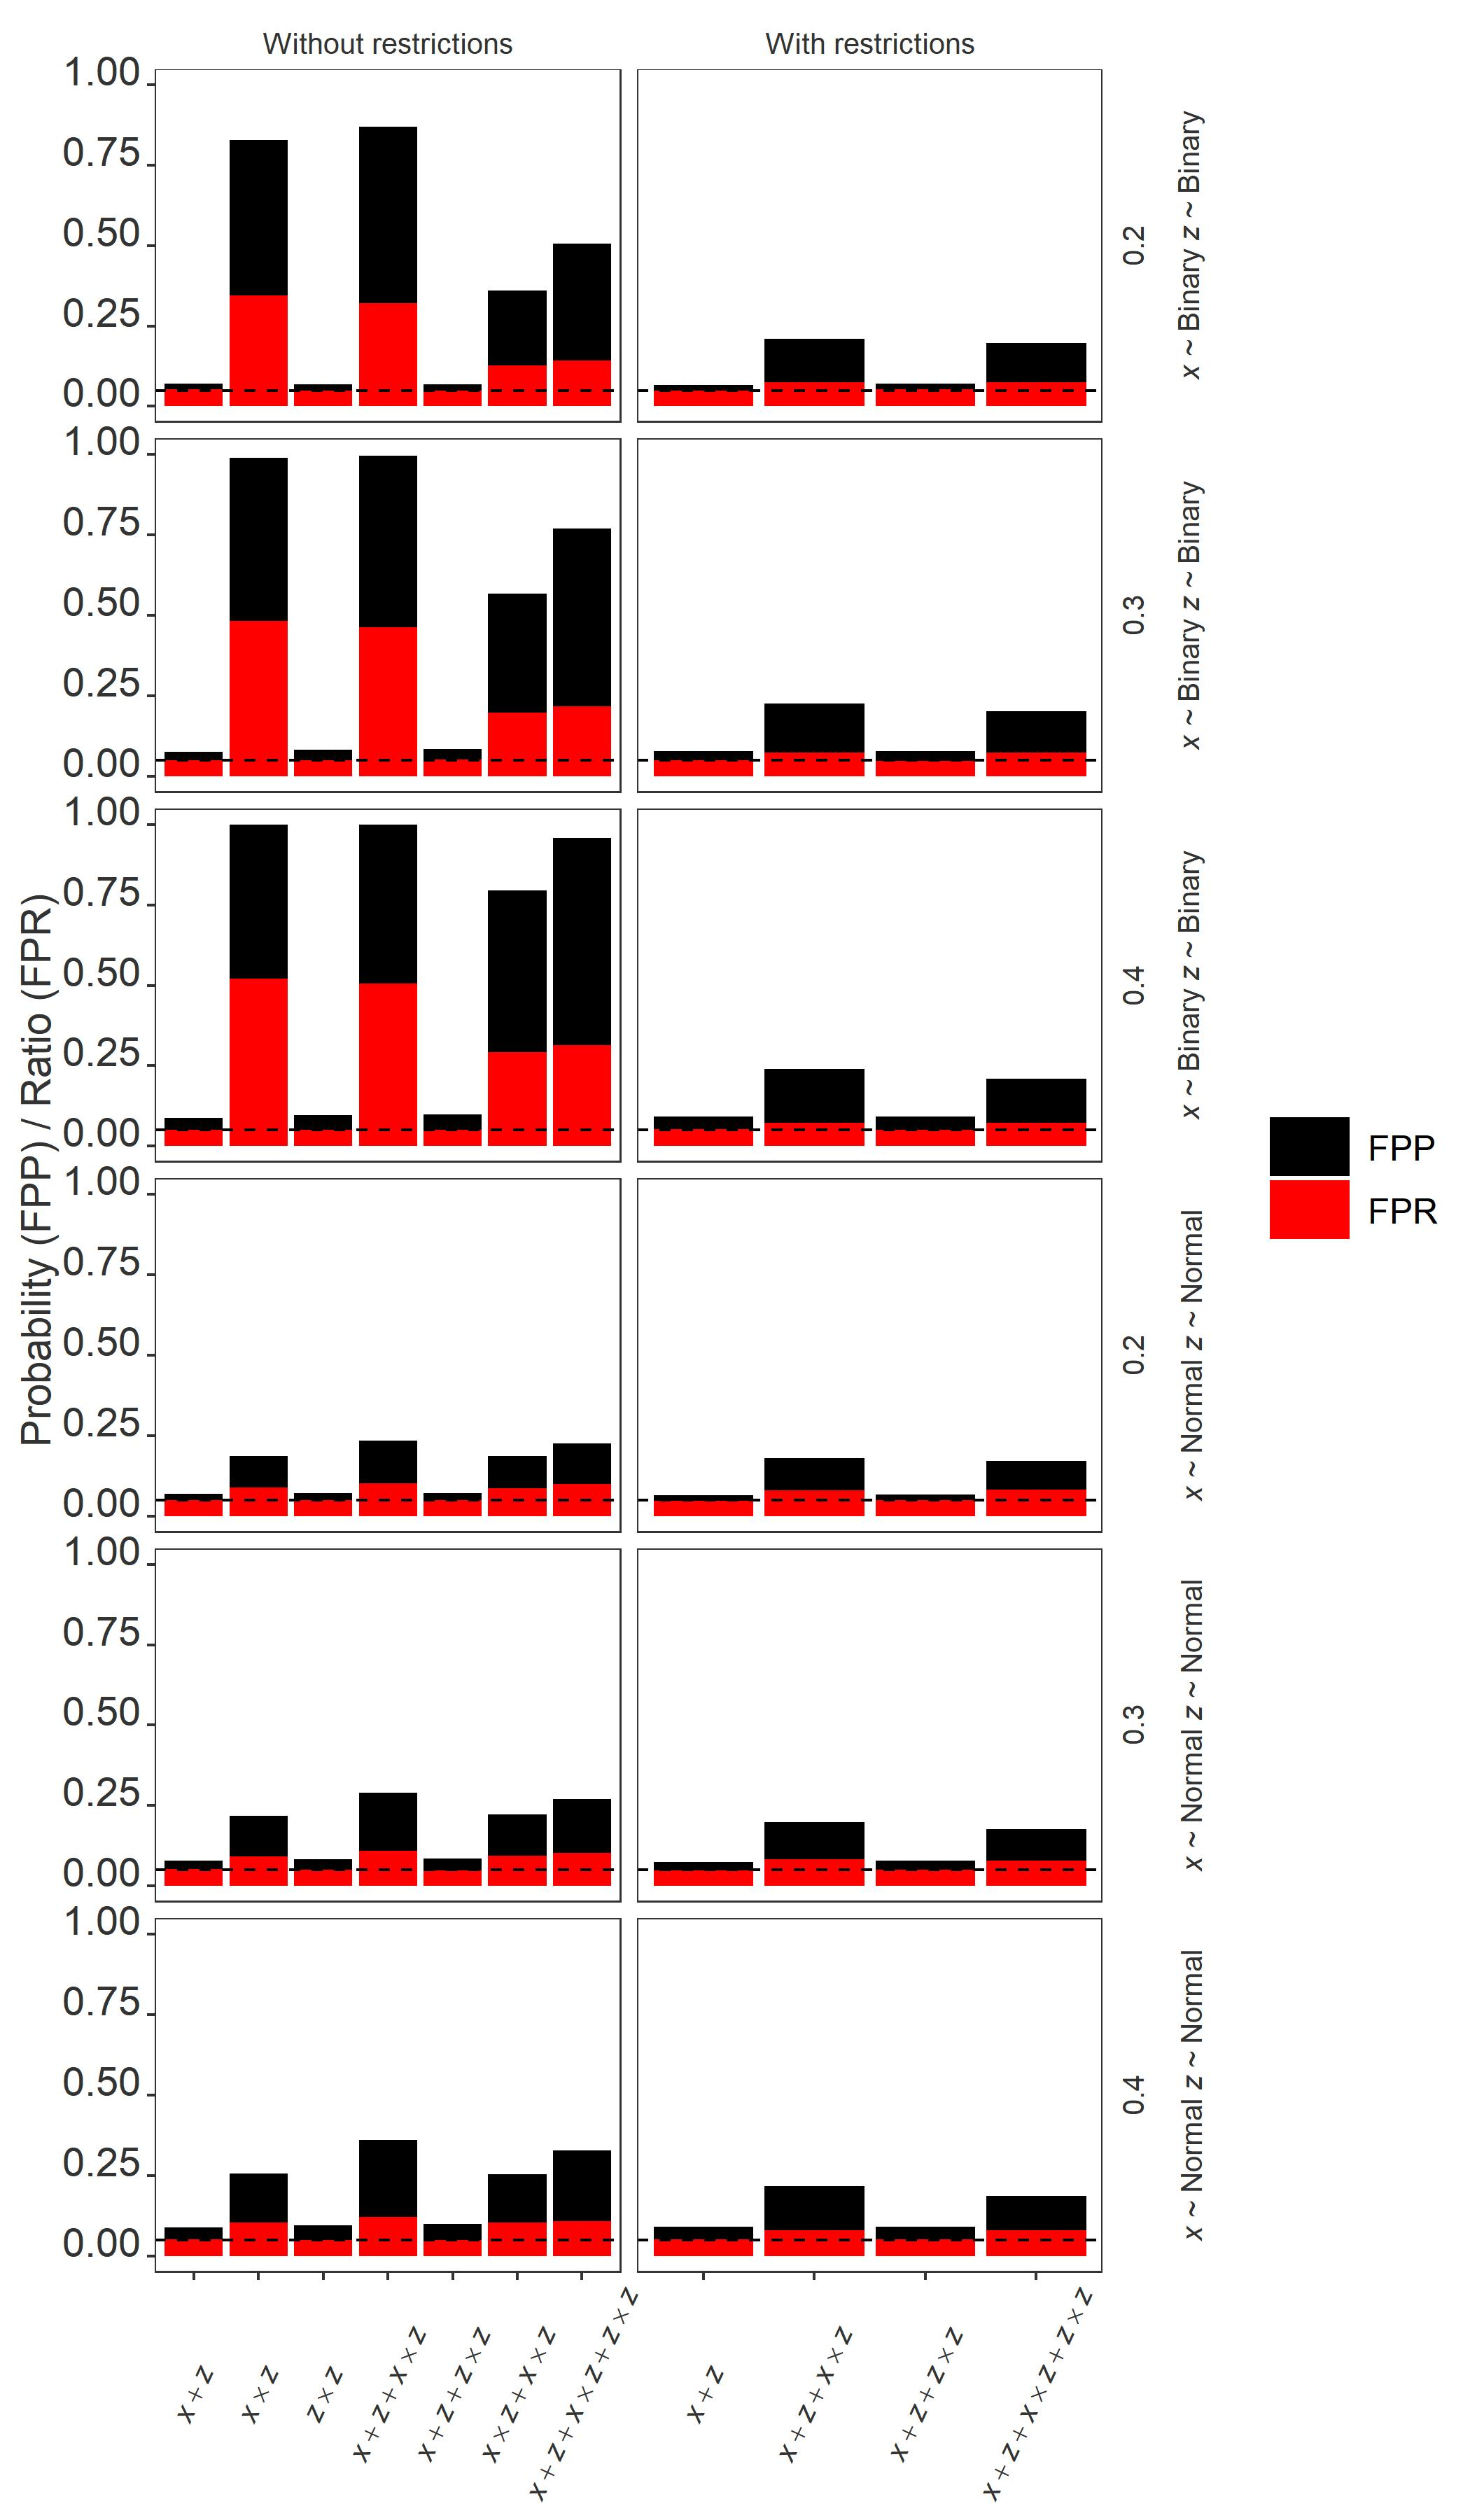
\includegraphics{R/Analysis/Result/Figures/Figure2SI.jpeg}
\centering
\caption{Black is the FPP and red is FPR.  Increased effect of having a higher correlation for the different sets}
\label{fig:mainfigure}
\end{figure}

\begin{figure}[ht]
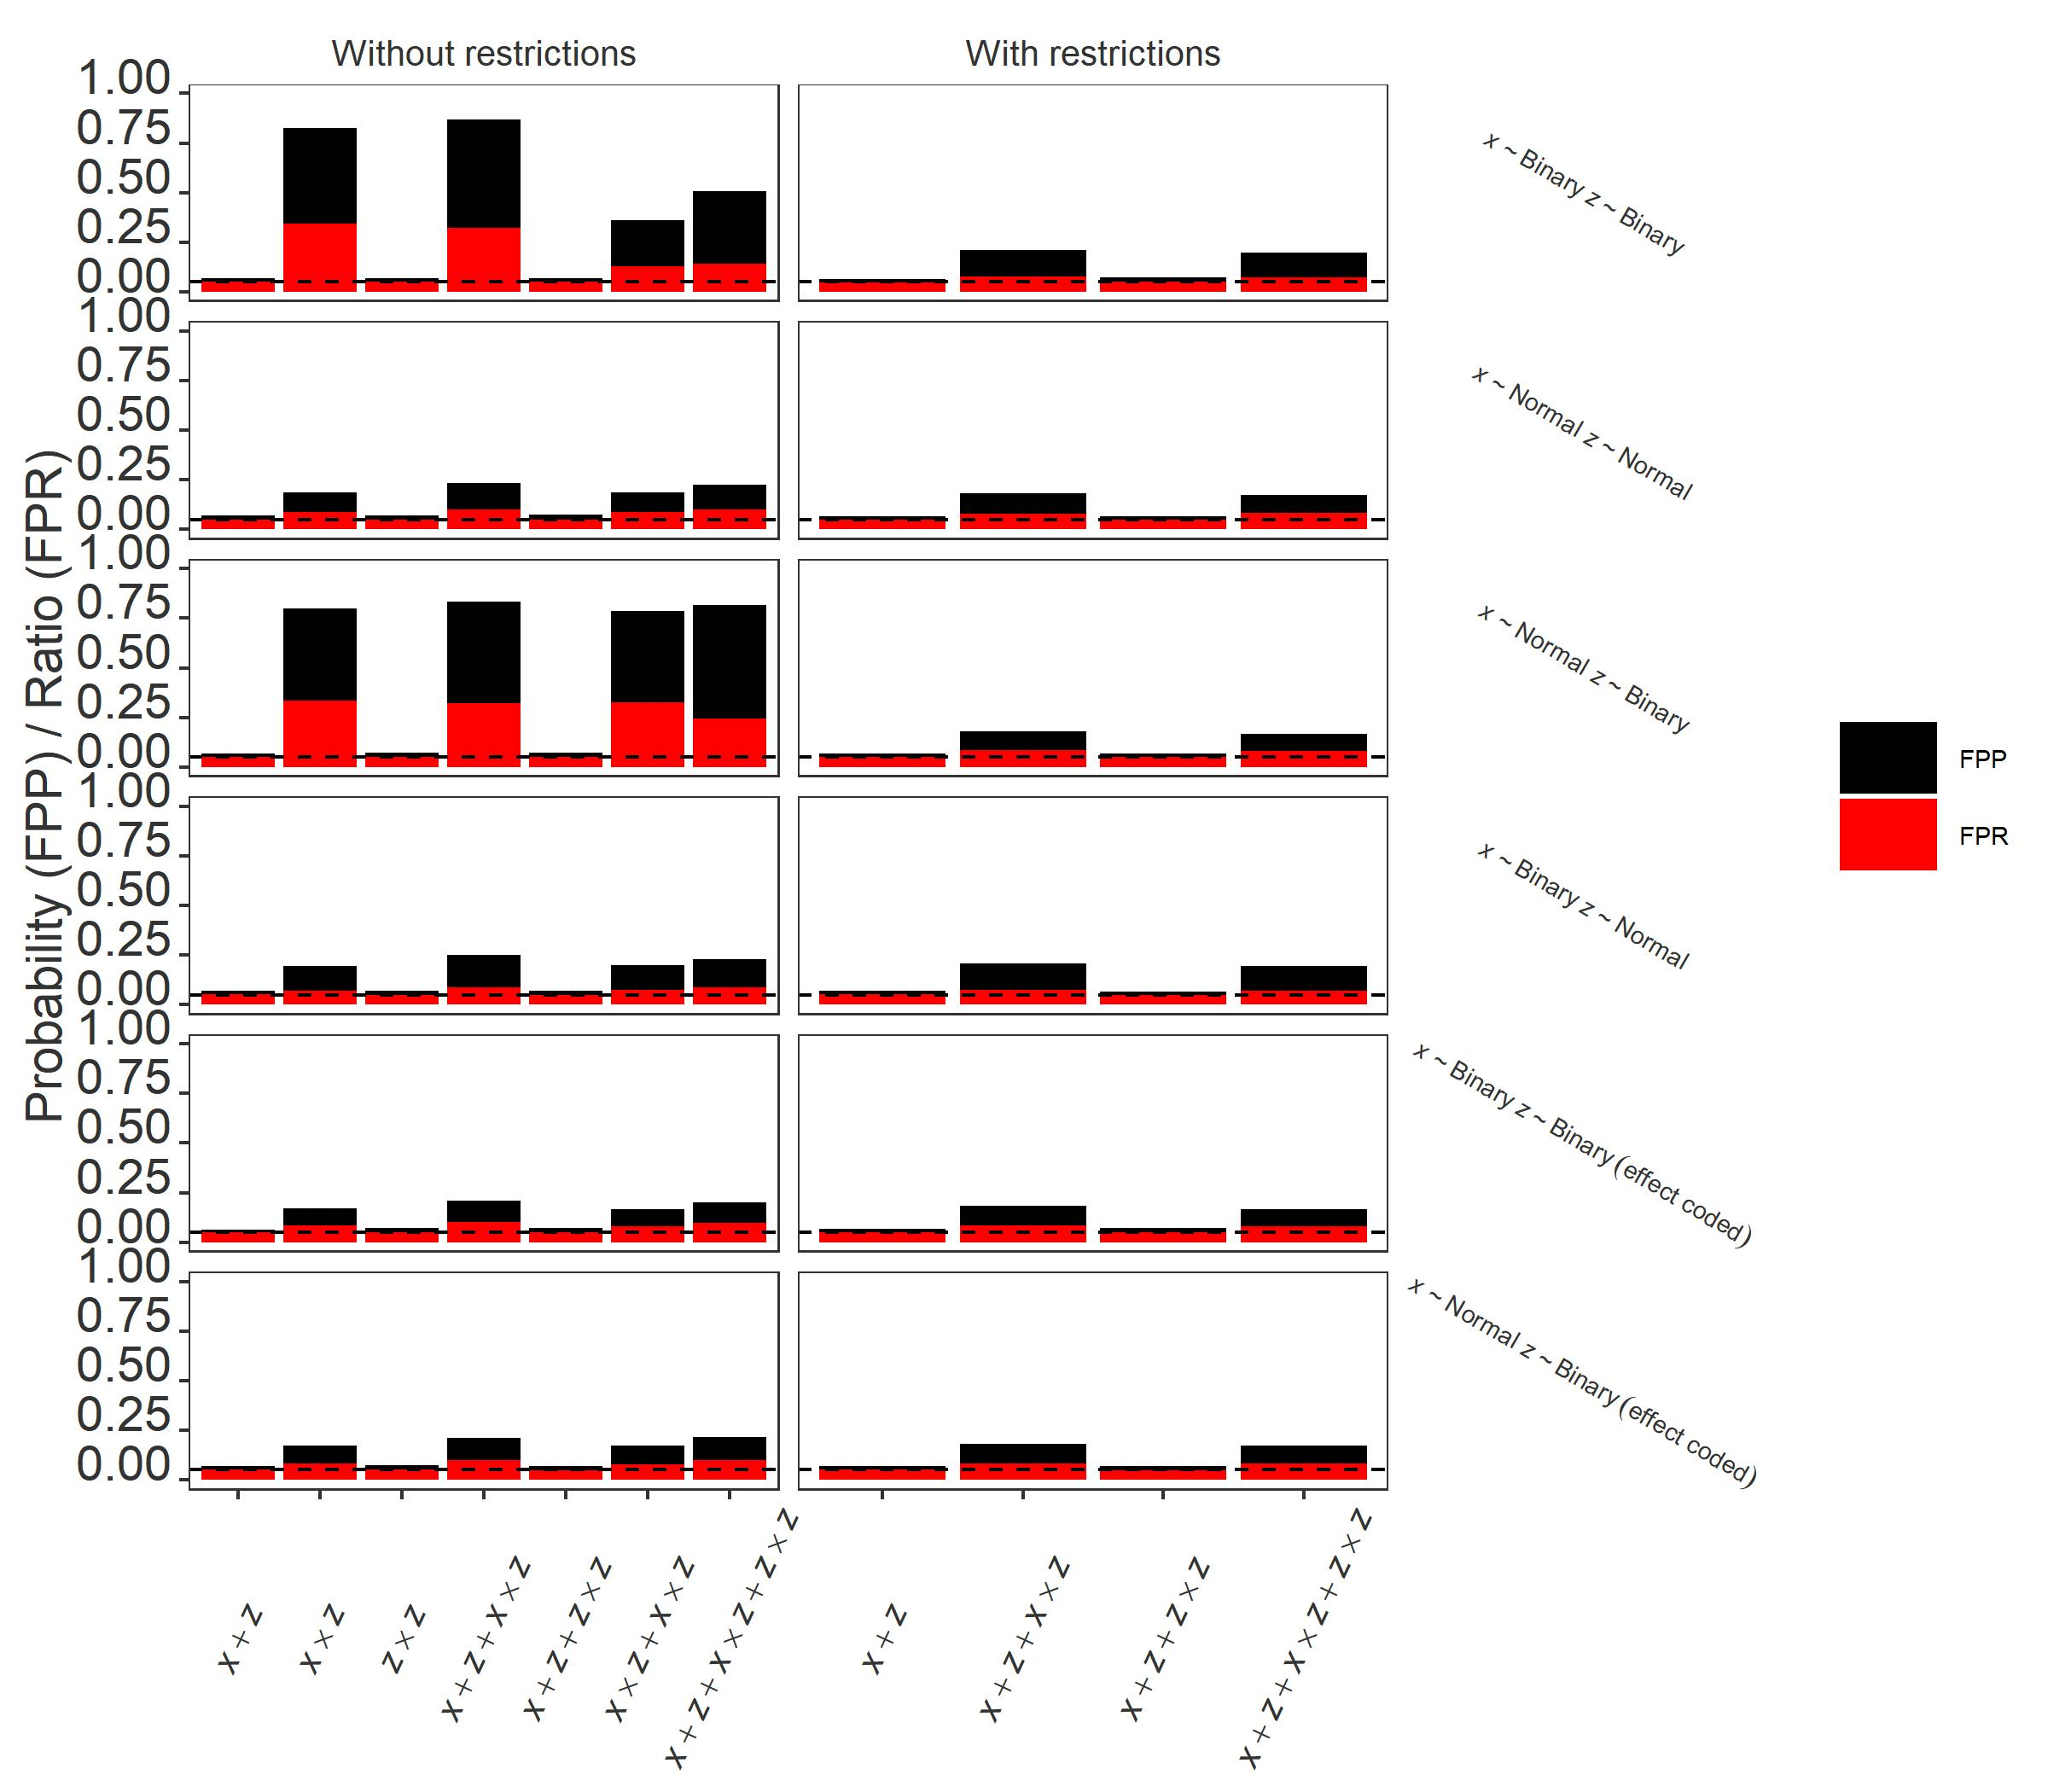
\includegraphics{R/Analysis/Result/Figures/Figure1ASI.jpeg}
\centering
\caption{Black is the FPP and red is FPR.  Here for all combinations of data distribution. The description of the figure is otherwise the same as for Figure 1}
\label{fig:mainfigure}
\end{figure}

\begin{figure}[ht]
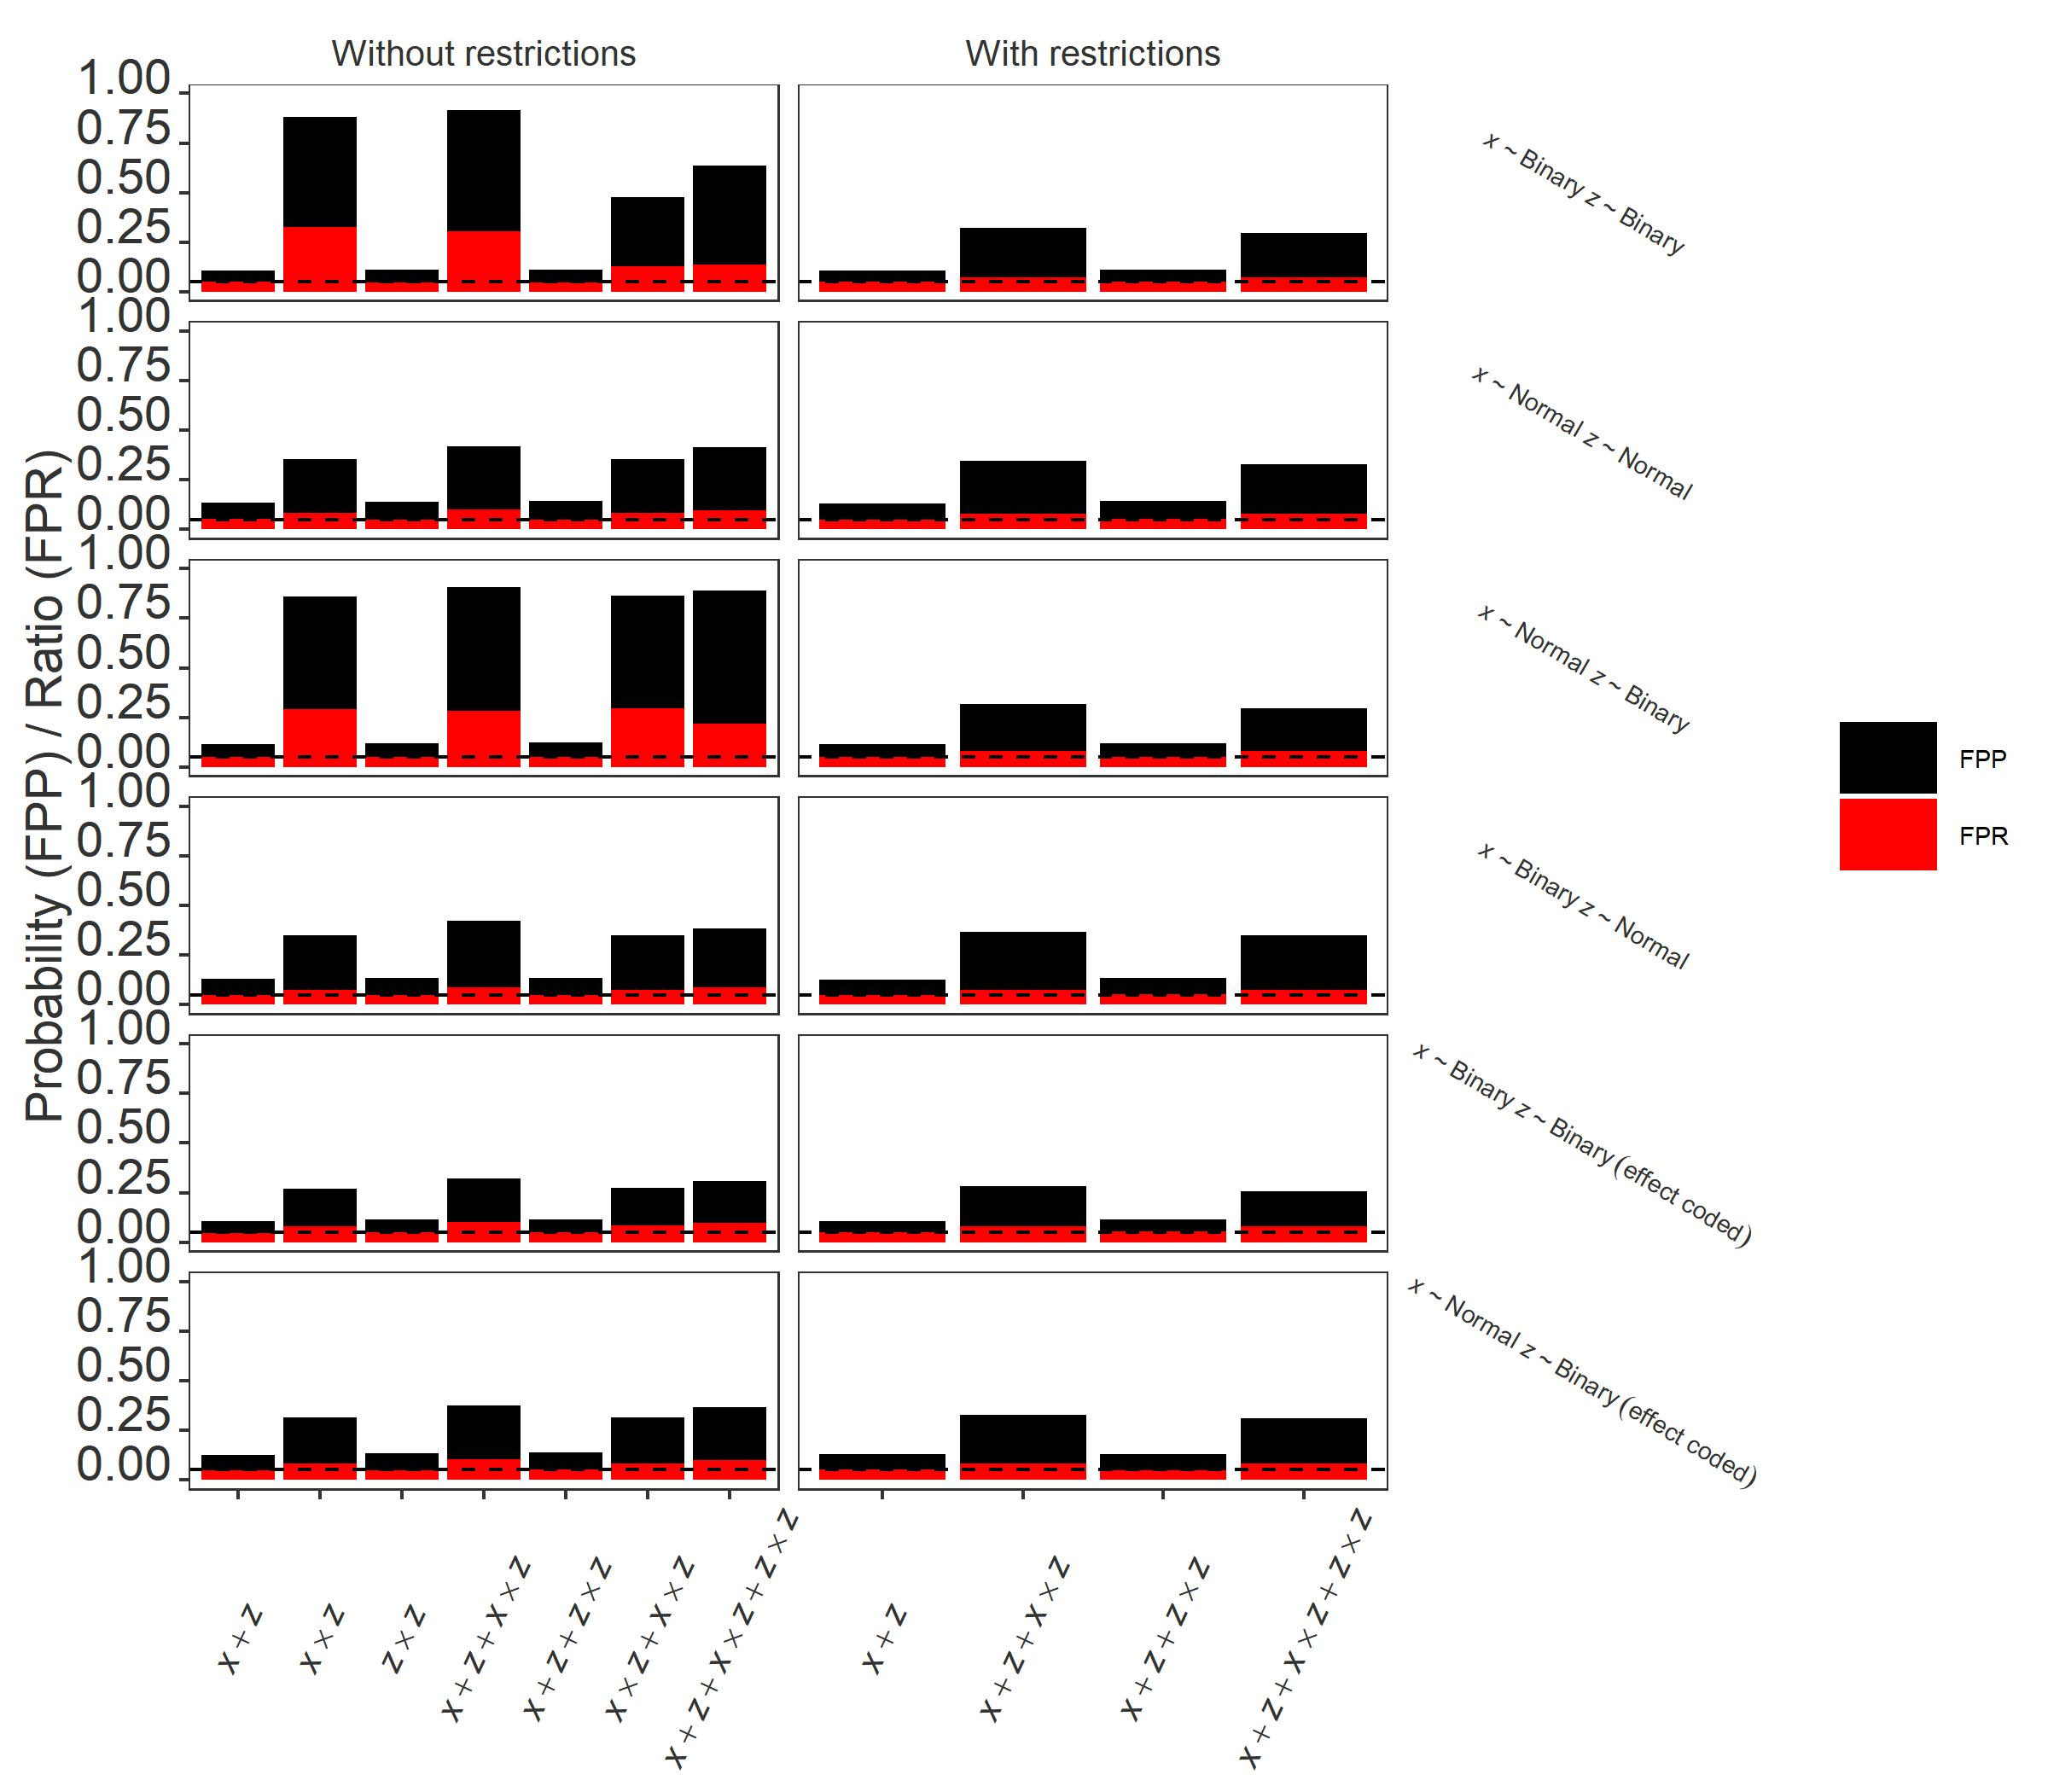
\includegraphics{R/Analysis/Result/Figures/Figure1BSI.jpeg}
\centering
\caption{Added effect of using outlier criteria. Black denotes the FPP and red denotes the FPR. Here are shown  all combinations of data distributions (binary and continuous). The description of the figure is otherwise the same as for Figure 1.}
\label{fig:mainfigure}
\end{figure}

\begin{figure}[ht]
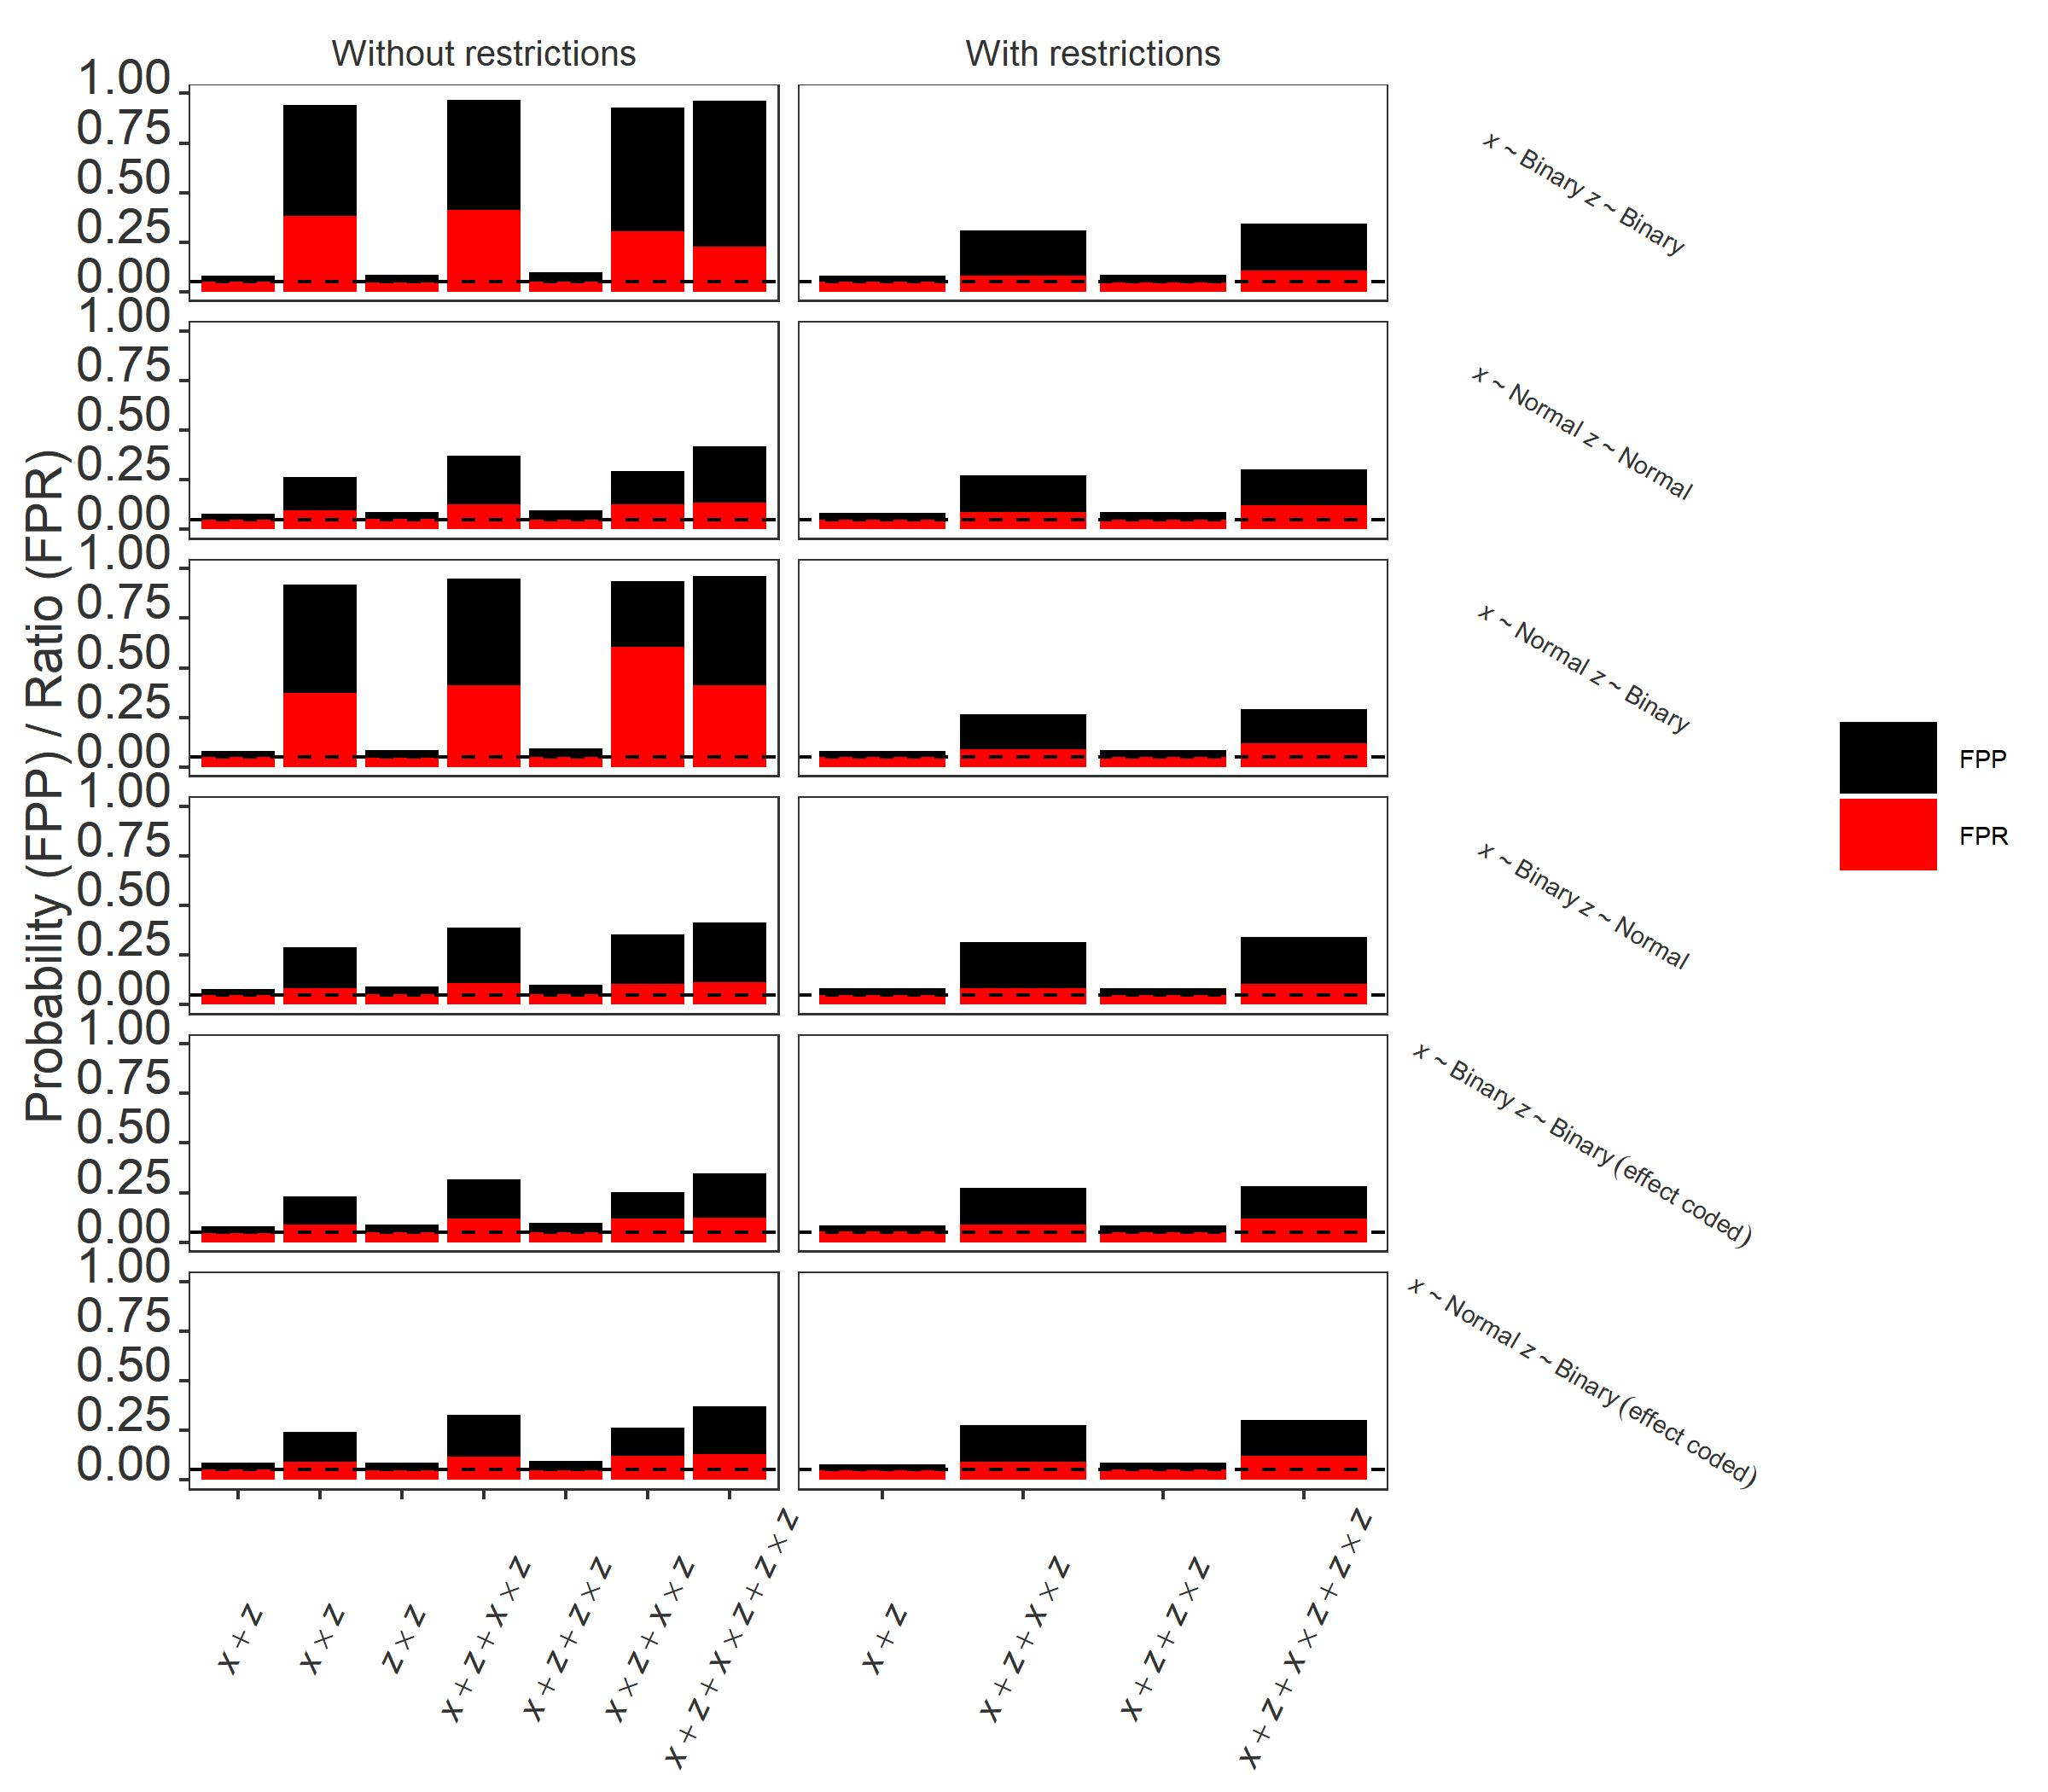
\includegraphics{R/Analysis/Result/Figures/Figure1CSI.jpeg}
\centering
\caption{Added effect of using one more covariate. Black is the FPP and red is FPR.  Here for all combinations of data distribution. The description of the figure is otherwise the same as for Figure 1}
\label{fig:mainfigure}
\end{figure}

\begin{figure}[ht]
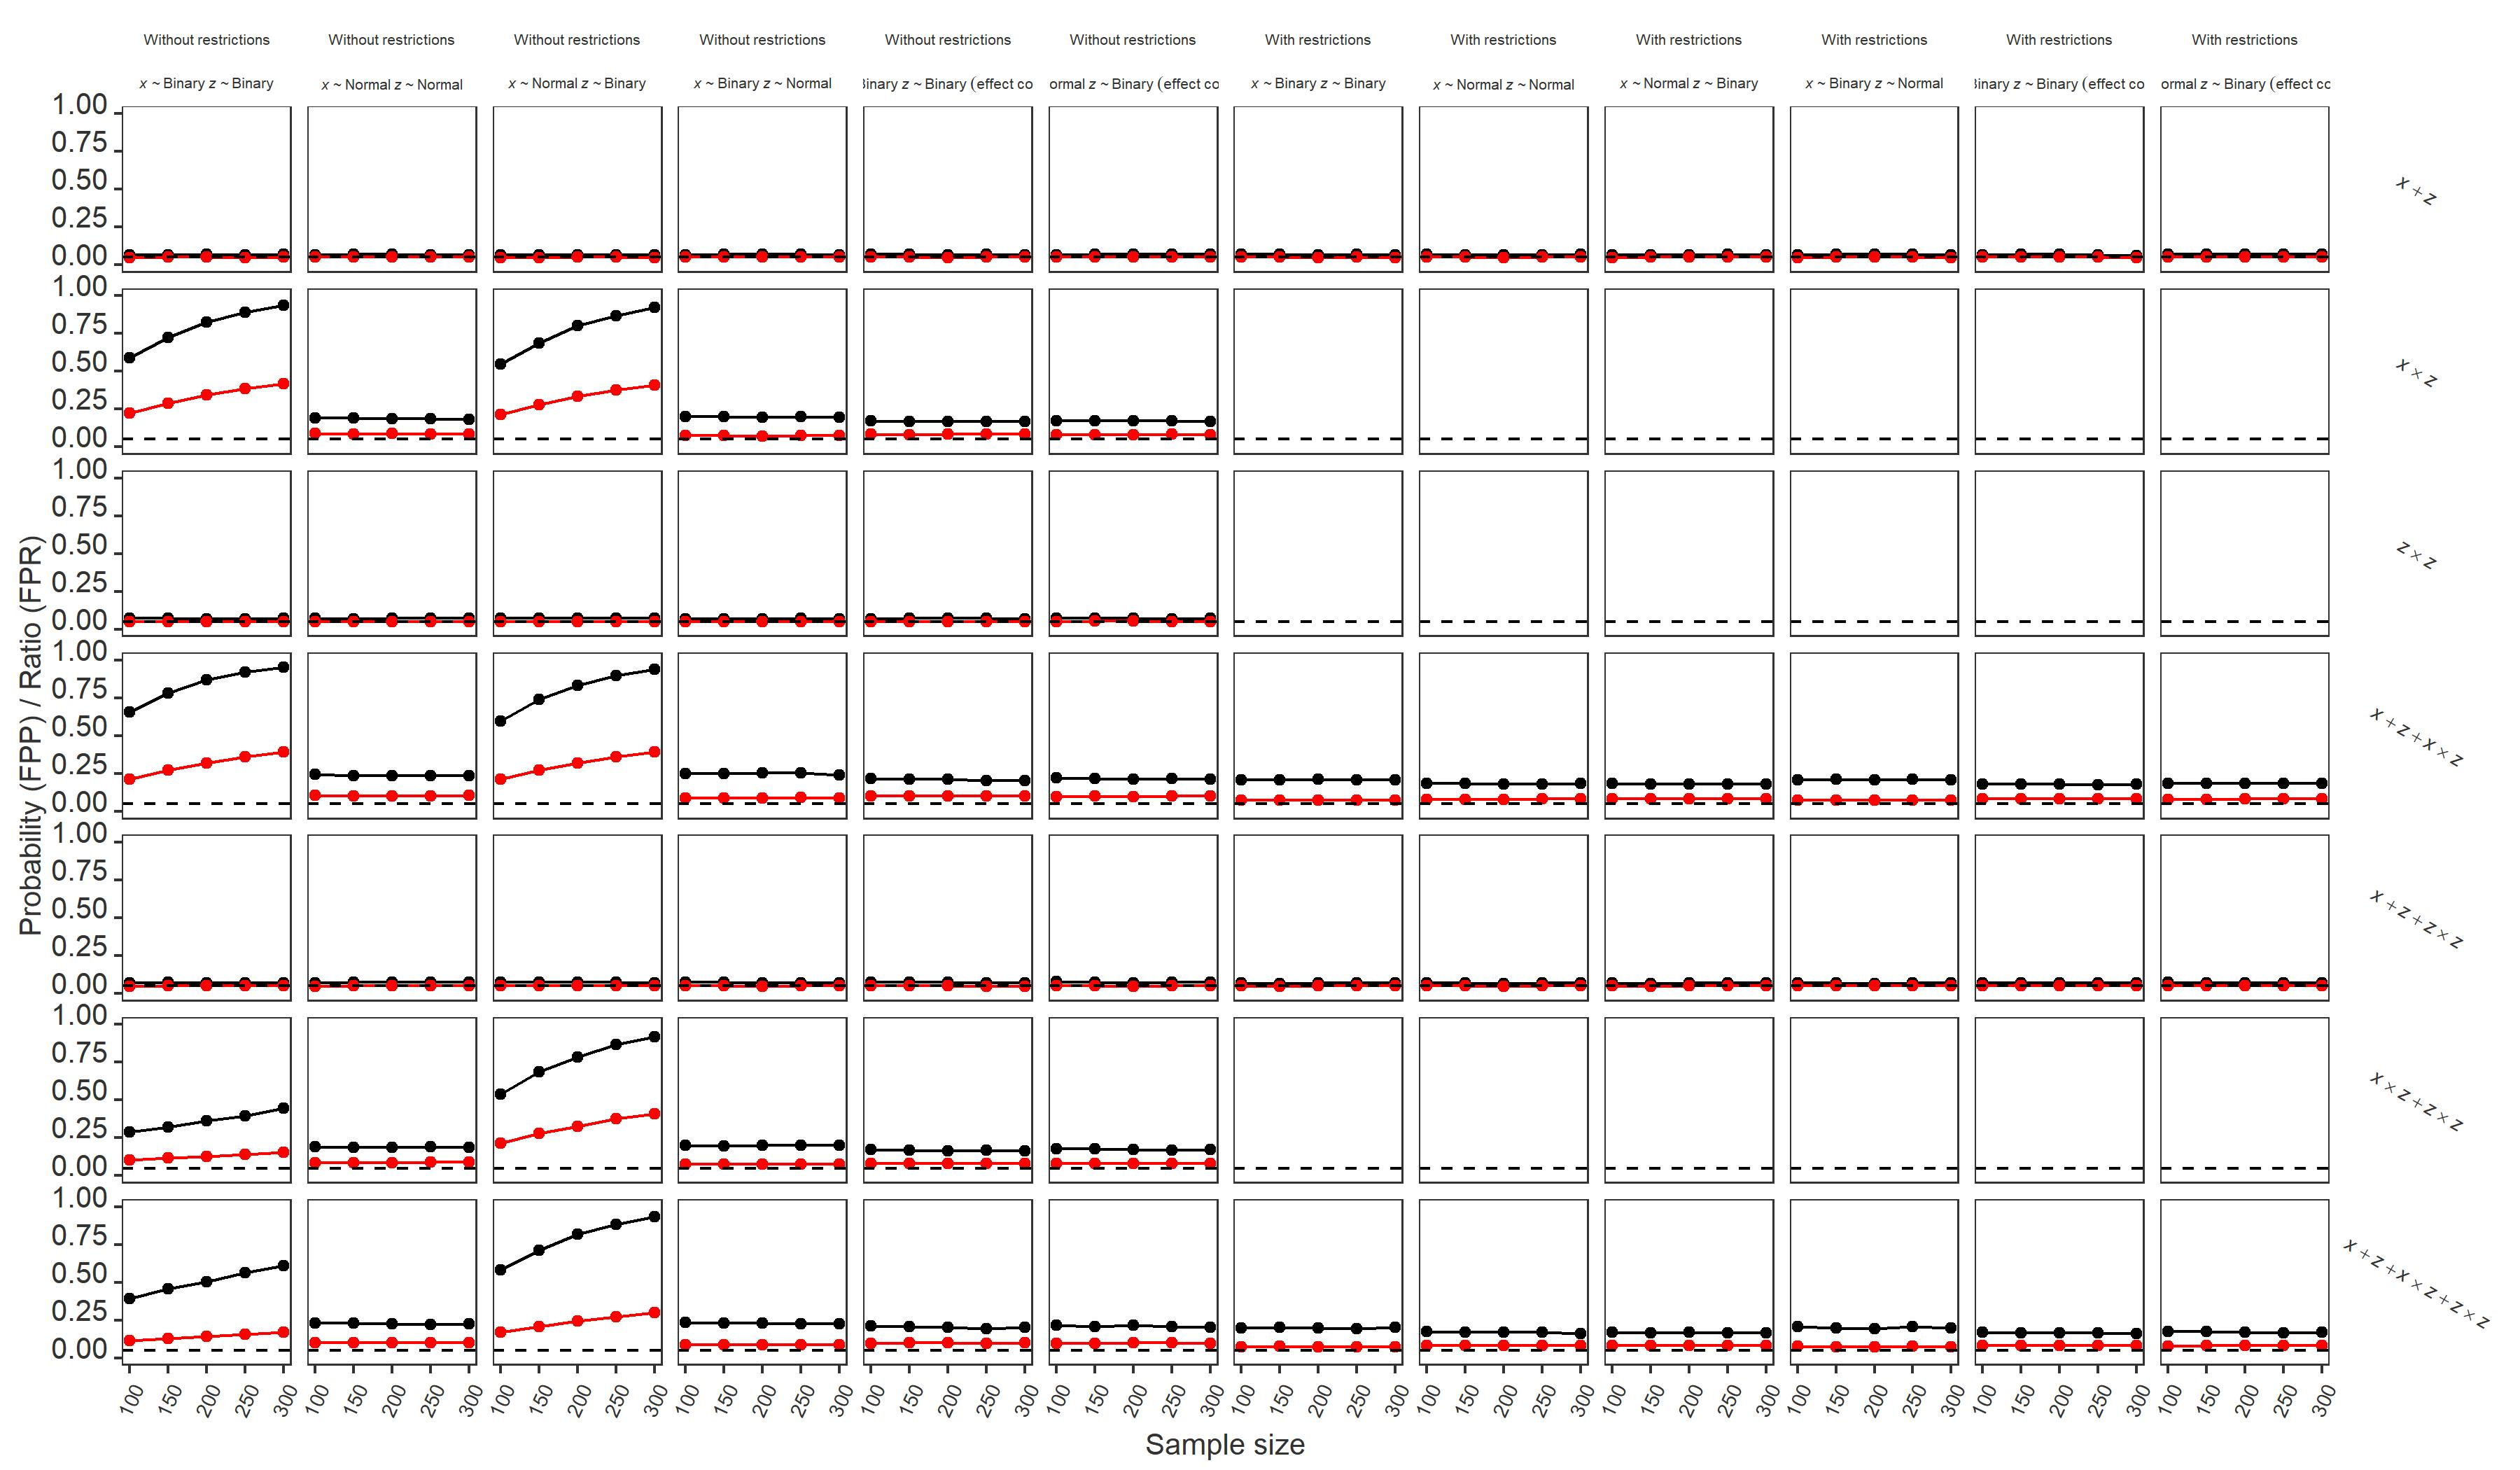
\includegraphics{R/Analysis/Result/Figures/Figure1DSI.jpeg}
\centering
\caption{Effect of increasing sample size. Black is the FPP and red is FPR.  Here for all combinations of data distribution. The description of the figure is otherwise the same as for Figure 1}
\label{fig:mainfigure}
\end{figure}

\begin{figure}[ht]
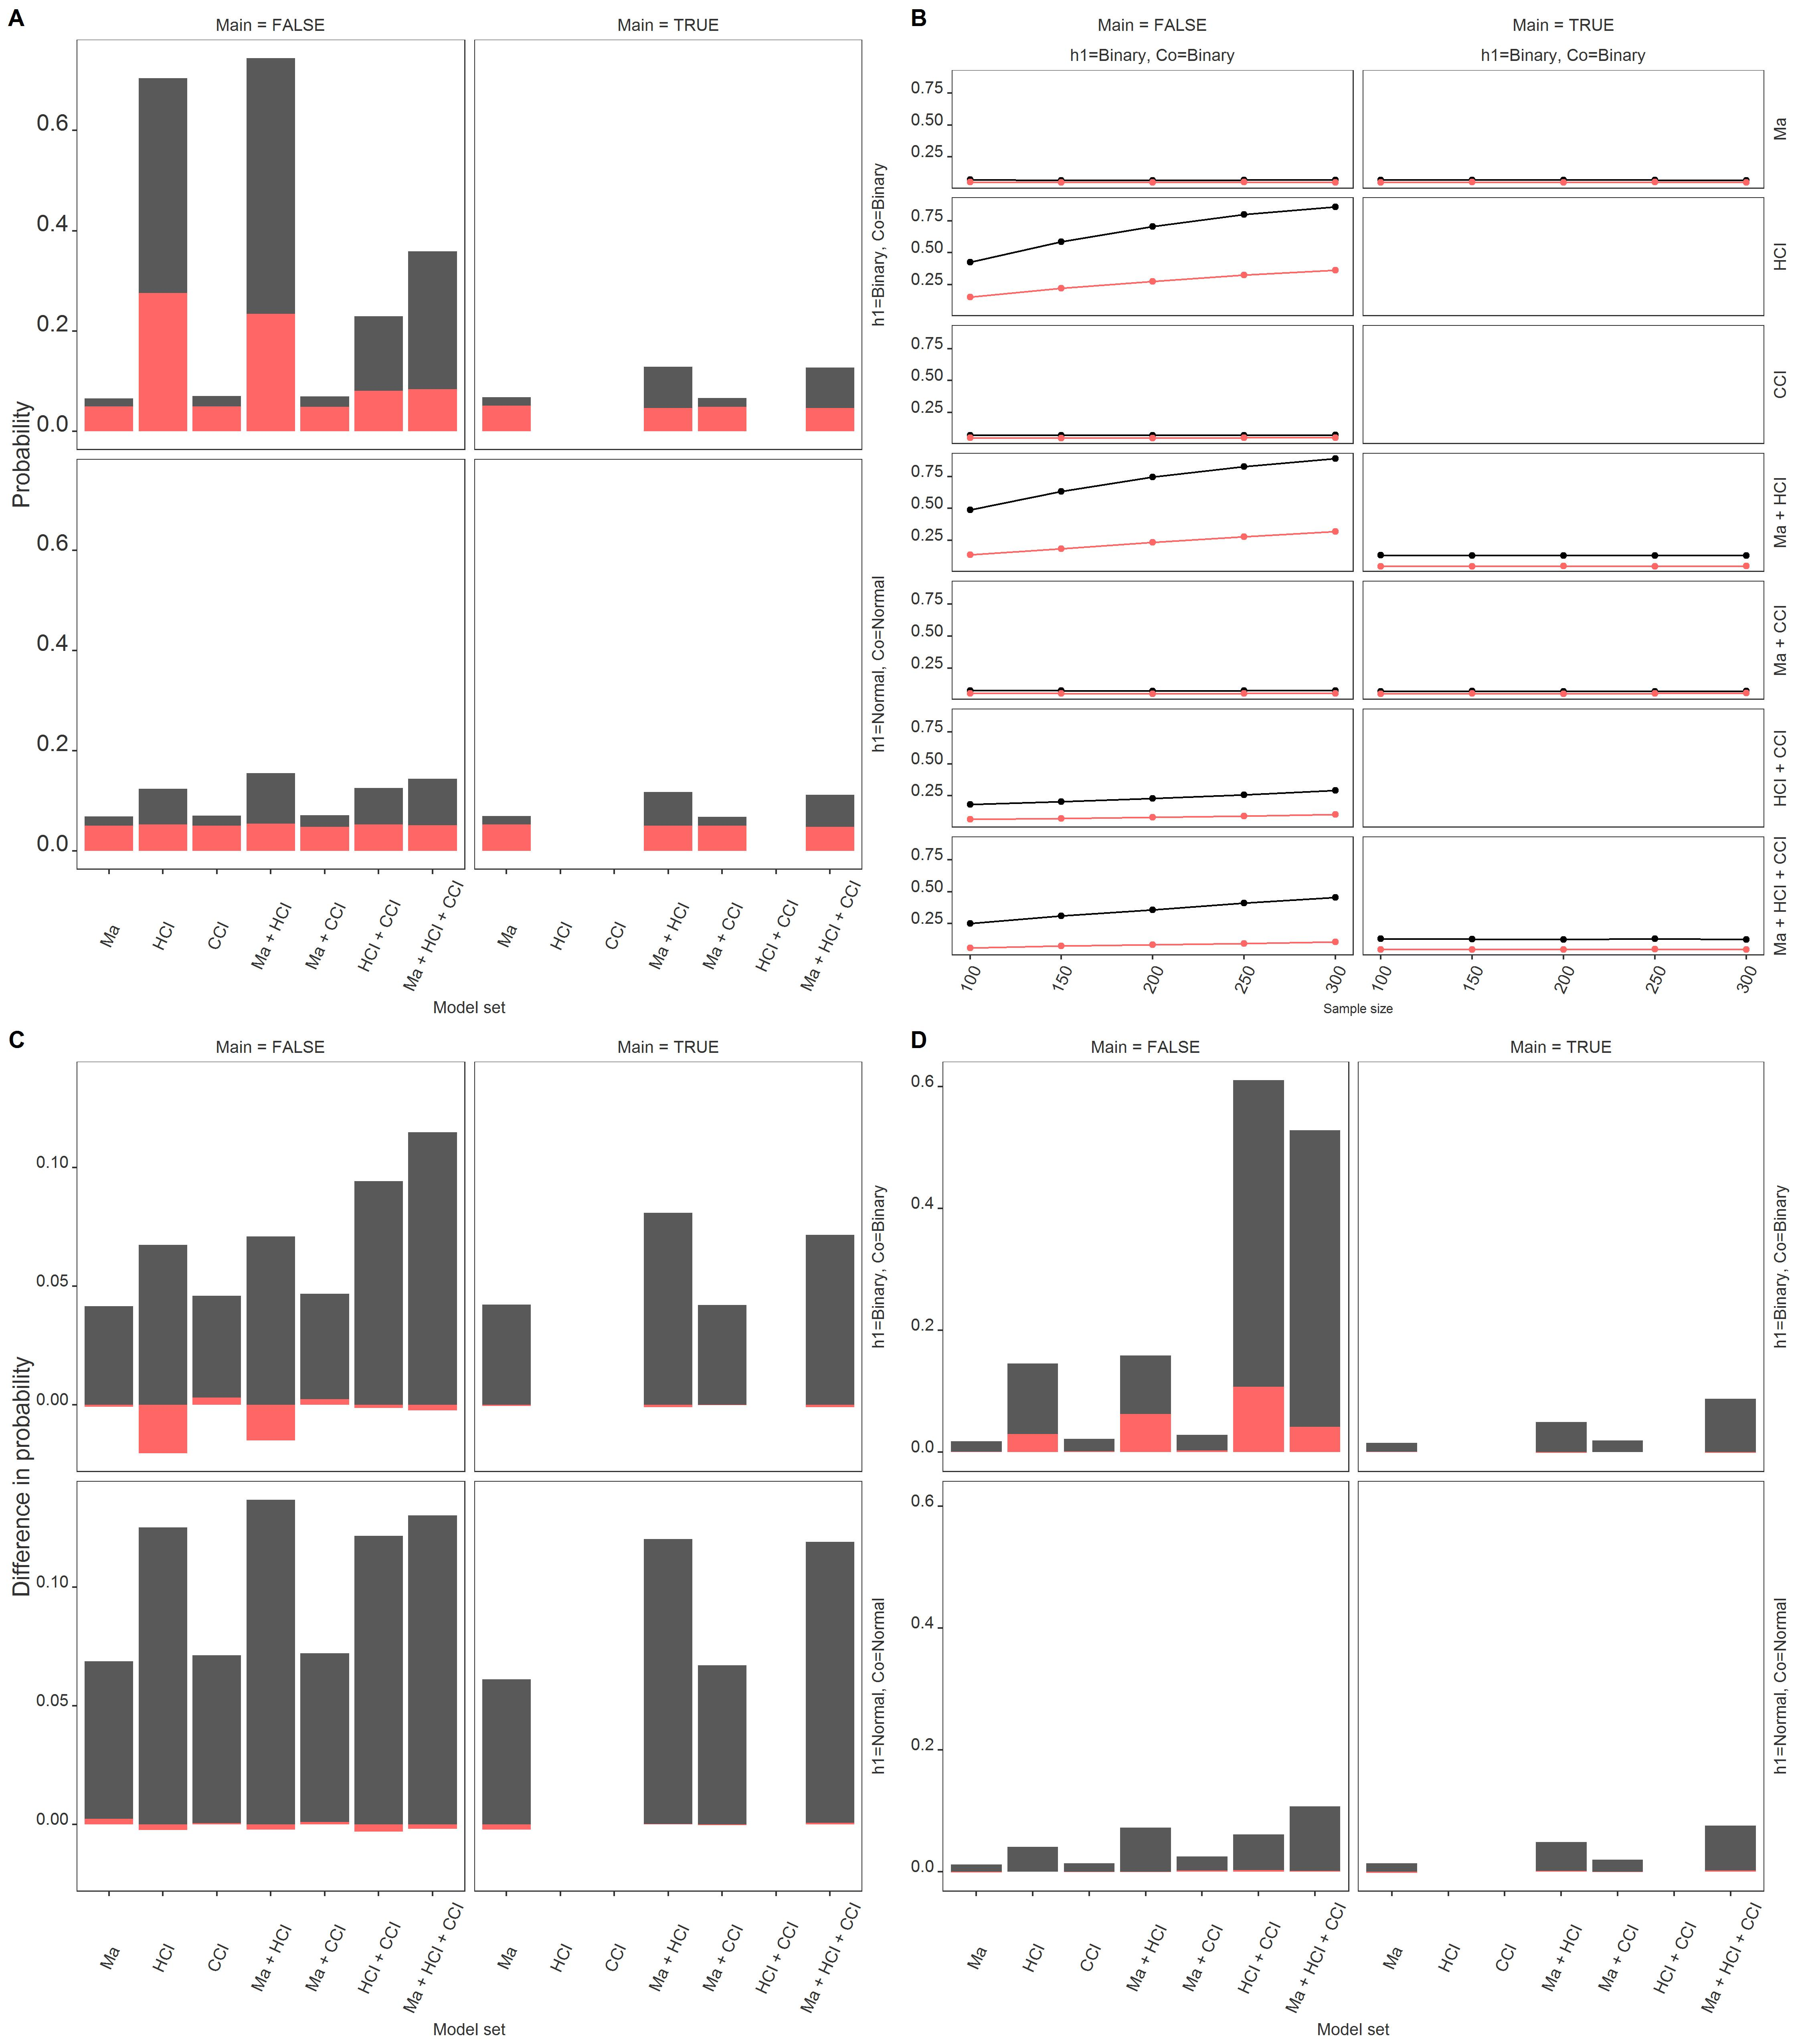
\includegraphics[width=0.8\textwidth]{R/Analysis/Result/Figures/Figure1BF.jpeg}
\centering
\caption{The figure shows the false-positive rate divided by model set and whether the main effects should follow the interactions or not. Black denotes the FPP and red denotes the FPR. The figures are otherwise the same as Figure 1-4 but with Bonferroni correction applied.}
\label{fig:mainfigure}
\end{figure}
